%=============================================================================
% CHAPTER 1: INTRODUCTION
%=============================================================================

\chapter{Introduction}

\section{Background and Motivation}

In the digital age, passwords remain the most common and accessible method people use to secure online accounts and protect sensitive information. Despite their widespread use, weak and reused passwords continue to represent one of the leading vulnerabilities exploited in modern cybersecurity incidents. Even with technological advances in authentication methods, such as biometrics, hardware tokens, or two-factor/multi-factor verification, the vast majority of online services still rely on traditional passwords as the first line of defence.

During my studies and everyday use of technology, I noticed that most users tend to underestimate the importance of password strength and good password hygiene. Many choose simple or predictable combinations such as ``123456'' or ``password,'' unaware that such passwords can be guessed in seconds by automated tools using dictionary attacks, brute-force techniques, or credential stuffing. In addition, users frequently reuse the same password across multiple platforms, meaning that a compromise of a single account can easily cascade into a much larger security incident. This widespread lack of awareness, combined with poor password management habits, contributes significantly to the increasing number of successful data breaches, identity thefts, and unauthorised account takeovers.

According to the Verizon Data Breach Investigations Report, approximately 80\% of hacking-related breaches involve compromised or weak credentials \cite{verizon2024}. The NordPass annual report on the most common passwords consistently shows that trivially guessable passwords such as ``123456,'' ``admin,'' and ``password'' dominate the top positions year after year \cite{nordpass2024}. These statistics underscore the persistent gap between the known best practices and the actual behaviour of everyday users.

\begin{figure}[H]
    \centering
    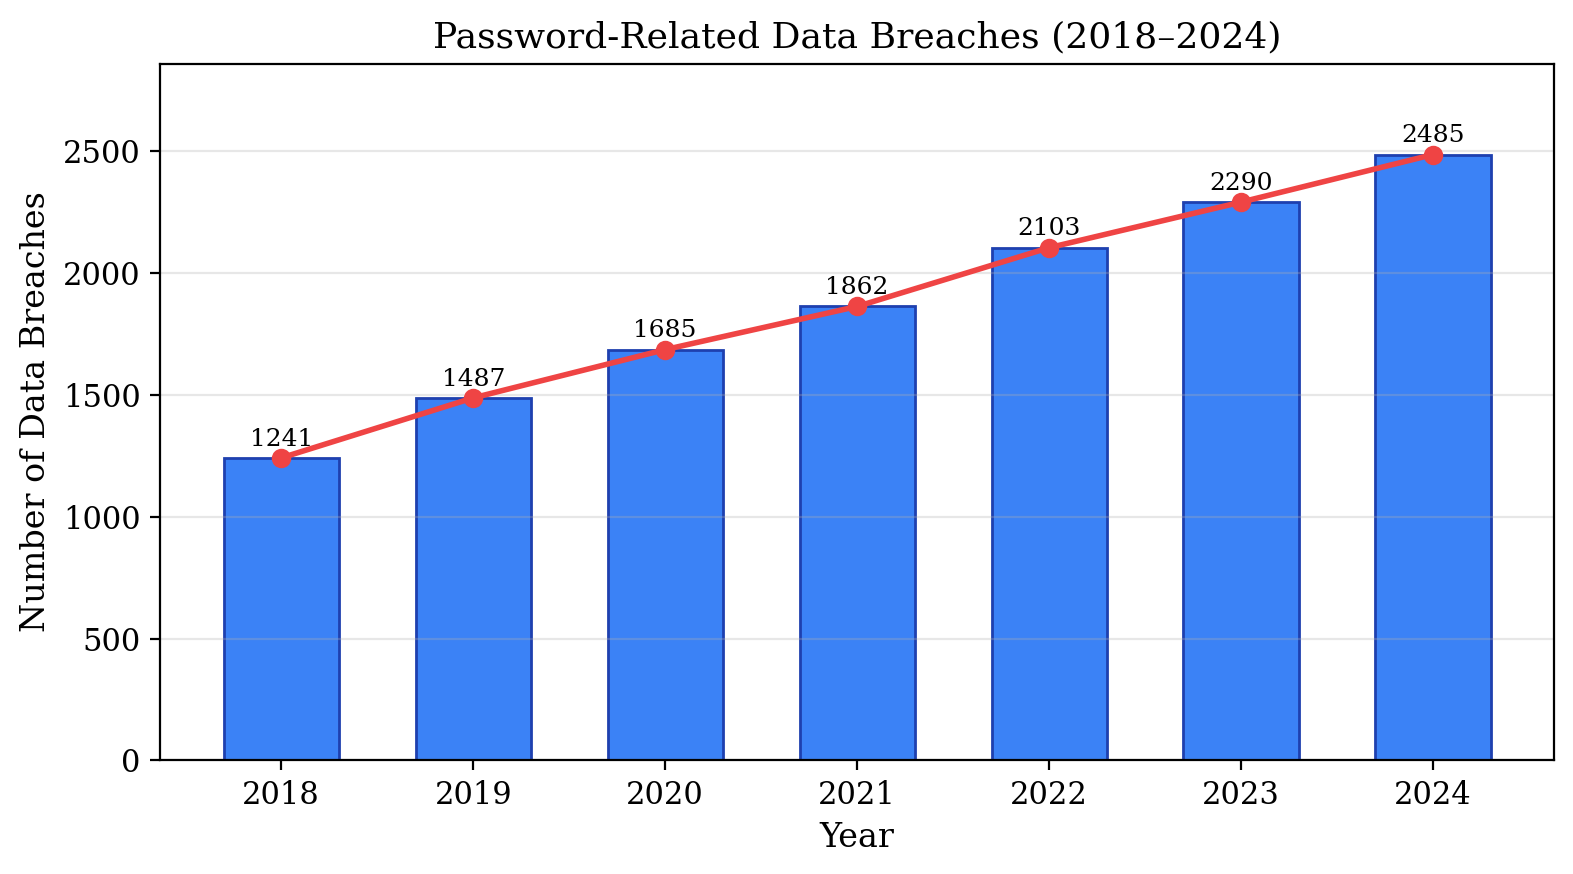
\includegraphics[width=0.85\textwidth]{figures/password_breach_trend.png}
    \caption{Trend of password-related data breaches from 2018 to 2024.}
    \label{fig:breach_trend}
\end{figure}

\begin{figure}[H]
    \centering
    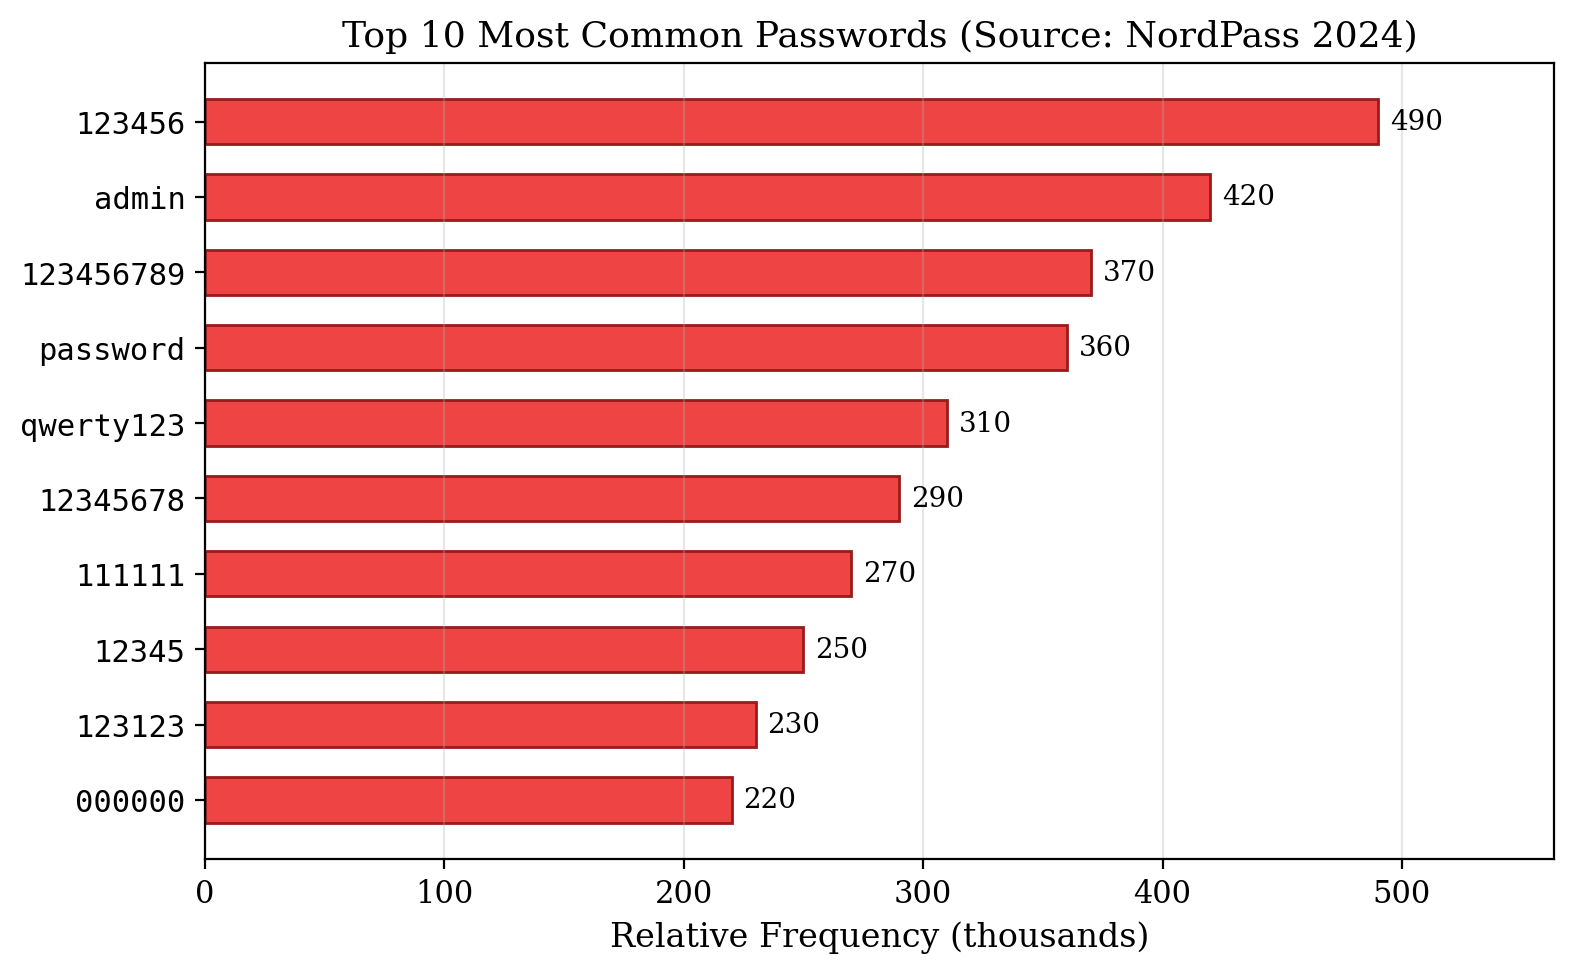
\includegraphics[width=0.85\textwidth]{figures/top_passwords_chart.png}
    \caption{Top 10 most common passwords and their usage frequency.}
    \label{fig:top_passwords}
\end{figure}

I have always been interested in practical applications of cybersecurity, especially in areas where user behaviour directly affects digital safety. For that reason, I decided to develop a password strength evaluation tool that helps users understand how secure their passwords are and how to improve them. The tool aims not only to give a numerical or qualitative strength rating, but also to provide clear, actionable feedback on issues such as length, character diversity, resistance to common attack patterns, and susceptibility to known leaked-password lists.

The project combines both theoretical knowledge about password security—such as entropy, common attack vectors, and best-practice guidelines from standards like NIST— with the practical skills I have gained in Python programming, including modular software architecture, secure handling of user data, graphical interface design, and implementation of hybrid security checks. Through this work, I aim to raise awareness of secure password practices and contribute to a safer online experience for everyday users.


\section{Aim of the Thesis}

The main aim of my thesis is to design, implement, and evaluate a Python-based desktop application with a graphical user interface and real-time hybrid analysis that can assess the strength of user passwords and provide constructive, user-friendly feedback. Through this project, I intend to demonstrate my ability to analyse a real-world cybersecurity problem, design an algorithmic solution based on established security principles and current best practices, and implement it as a functional, maintainable, and extensible tool that can be realistically deployed in contemporary computing environments.

Specifically, the objectives of the thesis are to:
\begin{itemize}
    \item analyse common patterns and weaknesses that make passwords insecure, including predictable structures, reuse of credentials across multiple services, use of personal or easily guessable information, and susceptibility to automated attacks,
    \item develop a hybrid algorithm that assesses password strength based on five measurable dimensions---length, character diversity, entropy, pattern detection, and dictionary comparison---while keeping the model transparent and interpretable to end users through named scoring constants and clear feedback,
    \item identify dictionary words and common patterns (such as keyboard sequences, reversed keyboard patterns, repeated or sequential characters, leetspeak variants, and predictable substitutions) that lower security, and incorporate these findings into the scoring and feedback mechanism,
    \item design a dark-themed graphical user interface with CustomTkinter that provides real-time password analysis through a debounced input mechanism, animated visual indicators, and a two-column analysis layout that presents both a score overview and detailed improvement suggestions simultaneously,
    \item implement an iterative improvement process, documented through 18 systematic enhancements and a user-experience redesign, demonstrating that structured quality refinement leads to a measurably better tool,
    \item generate meaningful, context-aware feedback to help users create stronger passwords by suggesting specific improvements and explaining the underlying security rationale in clear, non-technical language, with suggestions originating from the evaluation engine to ensure a single source of truth,
    \item validate the effectiveness, robustness, and usability of the proposed evaluation method through functional testing on representative password samples, comparative analysis with existing password-strength meters, and a usability self-evaluation based on Nielsen's heuristics,
    \item document design decisions, limitations, and potential security and privacy concerns (such as safe handling of input passwords) to inform future extensions and responsible use of the tool.
\end{itemize}

The purpose of the system is educational as well as practical---to raise user awareness of password security through an easy-to-use, self-contained tool that can be integrated into introductory cybersecurity training, personal use, or small-scale organisational environments. In addition, the system is intended to serve as a reference implementation that can be adapted or extended in future work, for example by incorporating machine-learning-based estimators, support for passphrases, or integration into web and mobile authentication workflows.


\section{Scope of the Thesis}

The thesis comprises both a theoretical and a practical component. The theoretical part examines the foundations of password security, including threat models, common attack methods (such as brute-force, dictionary, and credential-stuffing attacks), and the mathematical concepts used to measure password robustness, such as entropy, search space, and estimated attack complexity. It also reviews existing password-strength evaluation approaches and guidelines from recognised standards (e.g.\ NIST recommendations and relevant industry best practices) to situate the proposed tool within the broader context of password security research and practice. Where appropriate, the limitations and known shortcomings of current approaches are discussed in order to motivate specific design choices made in this work.

The practical part focuses on the development process of the proposed tool, including requirements analysis, modular architectural and interface design decisions, algorithm implementation, and both functional and non-functional testing, followed by a systematic evaluation. The implementation is built as a Python desktop application using CustomTkinter for the graphical user interface, featuring a dark-themed dashboard with real-time analysis via a 300\,ms debounced input mechanism, a two-column analysis layout, animated semicircular gauge and horizontal meter bar, and a cryptographically secure password generator. Particular attention is paid to code quality, modularity, performance, and maintainability, as well as the ease with which the tool can be adapted or extended (for example, to new dictionaries, language-specific patterns, or additional attack models). The development followed an iterative process of 18 systematic enhancements and a user-experience redesign, which is documented in detail.

I deliberately limit the project's scope to password strength evaluation and do not address topics such as encryption algorithms, password storage mechanisms (e.g.\ hashing and salting), multi-factor authentication, federated identity management, or large-scale authentication infrastructures. These subjects are important and closely related areas of cybersecurity but fall beyond the intended scope of a first-cycle practical project and would require separate, dedicated treatment and substantially broader technical coverage.

\clearpage

\section{Justification of the Topic Choice}

I chose this topic because it allows me to apply theoretical cybersecurity knowledge in a way that produces a tangible, working result. The password strength evaluator represents a concrete example of how programming and security theory can directly contribute to improving digital safety in everyday scenarios. It also enables me to demonstrate key skills---problem analysis, requirements engineering, algorithmic design, software implementation, documentation, and empirical evaluation---all of which are crucial in my field of study and highly valued in professional practice.

Moreover, the topic remains highly relevant. Data breaches caused or facilitated by weak, reused, or predictable passwords continue to occur regularly, affecting both individuals and organisations across different sectors \cite{verizon2024}. Despite the availability of advanced authentication methods (such as hardware tokens and biometric systems), passwords remain the dominant mechanism for user authentication on most systems and services. Accessible tools that educate users, help them understand the limitations of their current password choices, and encourage better practices are therefore needed more than ever.

\subsection{Contribution to Society}

Beyond personal skill development, this project addresses a genuine societal problem: the persistent gap between cybersecurity best practices and everyday user behaviour. The tool contributes to society in several concrete ways:

\begin{itemize}
    \item \textbf{Increasing user awareness:} By providing immediate, context-aware feedback as users type their passwords, the tool educates them about the specific weaknesses in their choices. Each suggestion explains not only \textit{what} to change but also \textit{why}---for example, ``Avoid keyboard patterns like qwerty or asdf---these are in every cracking dictionary.'' This educational approach helps users internalise good password practices rather than merely following rules mechanically.

    \item \textbf{Preventing common attacks through education:} The tool's hybrid evaluation model explicitly addresses the three most common password attack strategies---brute-force (through length and entropy scoring), dictionary attacks (through dictionary comparison and Levenshtein similarity), and pattern-based attacks (through sequential, repeated, and keyboard pattern detection). By making users aware that these attack strategies exist and that their passwords are vulnerable to them, the tool encourages the creation of passwords that resist all three.

    \item \textbf{Promoting better password hygiene:} The actionable suggestions and the integrated ``Generate Strong Password'' feature encourage users to move beyond simple, reused passwords toward stronger, unique credentials. The real-time feedback loop---type, evaluate, improve, re-evaluate---makes the process of strengthening a password feel natural and achievable rather than burdensome.

    \item \textbf{Providing a privacy-friendly alternative:} Unlike most online password checkers, which require transmitting the password over the internet, this tool processes everything locally. No passwords are stored, logged, or transmitted at any point. This privacy-first design means that users can evaluate their most sensitive passwords without risking exposure to third-party services, a concern that has become increasingly important as data breaches continue to make headlines \cite{verizon2024}.

    \item \textbf{Democratising security knowledge:} The transparent scoring model, with its named constants and explainable breakdown, makes the evaluation process accessible to non-technical users. Unlike ``black box'' strength meters that provide a rating without explanation, this tool shows exactly how each dimension contributes to the final score, empowering users to make informed decisions about their password choices.
\end{itemize}

This project, while small in scale, aims to make a meaningful contribution to everyday cybersecurity awareness by providing a transparent, explainable password evaluation tool. The implementation emphasises interpretability, so that users not only receive a strength score but also understand the reasoning behind it and the specific changes that can improve their passwords. A distinctive contribution of this tool is its detection of reversed keyboard patterns---a weakness that most existing online password checkers fail to identify---demonstrating that even a compact, locally-run tool can offer analysis capabilities absent from some widely-used web-based checkers.

In addition to its immediate practical use, the tool can serve as a starting point for further work, such as integrating the evaluator into web applications, extending it to support multiple languages and cultural password patterns, combining it with password managers, or embedding it into broader security education initiatives and institutional security policies.

\clearpage

\section{Thesis Layout}

The structure of my thesis is organised as follows:
\begin{itemize}
    \item \textbf{Chapter 1} introduces the topic, defines the aim, scope, and motivation for the project.
    \item \textbf{Chapter 2} presents the theoretical background, including password vulnerabilities, mechanisms of password attacks, real-world breaches, entropy, existing evaluation techniques, and tools and standards.
    \item \textbf{Chapter 3} explains the methodology, system architecture, the hybrid evaluation algorithm, detection techniques, and the user interface approach.
    \item \textbf{Chapter 4} describes the implementation process, including project structure, the evaluation engine pipeline, core analysis modules, password generation, and the graphical interface.
    \item \textbf{Chapter 5} presents functional test results, a comparative analysis with existing tools, a usability self-evaluation, a discussion of advantages and disadvantages, and limitations.
    \item \textbf{Chapter 6} concludes the thesis with a summary of achievements, final conclusions, and possible future extensions.
\end{itemize}

%=============================================================================
% CHAPTER 2: THEORETICAL BACKGROUND
%=============================================================================

\clearpage

\chapter{Theoretical Background}

\section{Introduction}

Before I began designing my password strength evaluation tool, I first explored the theoretical and practical background of password security. Understanding how passwords are created, attacked, managed, and evaluated allowed me to identify the essential factors that determine their strength in real-world scenarios. This chapter summarises the key concepts, common attack methods, and established approaches to assessing password robustness, as well as the limitations of current practices.

In particular, I examine how users choose passwords, which psychological and usability factors influence those choices, and how attackers exploit predictable patterns. I also review existing metrics and tools for measuring password strength, including rule-based approaches, entropy-based models, and modern data-driven methods that leverage leaked password datasets. By outlining this foundation, the chapter motivates the design goals and requirements for my own evaluation tool.


\section{Role of Passwords in Our World}

Passwords serve as the primary mechanism for authentication in most systems people use, from email services to banking platforms, social networks, and cloud storage solutions. A password functions as a shared secret between the user and the system, serving as the first line of defence against unauthorised access. However, the effectiveness of this mechanism depends on password quality and how it is stored and verified by the system. Weak or reused passwords make it easier for attackers to compromise accounts, leading to identity theft, financial loss, data breaches, and large-scale compromise of online services.

In addition to attacks that directly guess or crack passwords, poor password practices---such as writing passwords on paper, sharing them between accounts, or using default credentials---further increase the risk. From an organizational perspective, compromised passwords can affect not only individual accounts but also critical infrastructure and sensitive business data.

Although advanced methods such as multi-factor authentication (MFA), hardware security keys, and biometrics are becoming more common, passwords still dominate due to their simplicity, low cost, and compatibility with existing systems. In many cases, they remain the fallback or recovery method even when stronger authentication is used. Figure~\ref{fig:auth_methods} illustrates the trade-off between adoption rate and security strength for the most common authentication methods.

\begin{figure}[H]
    \centering
    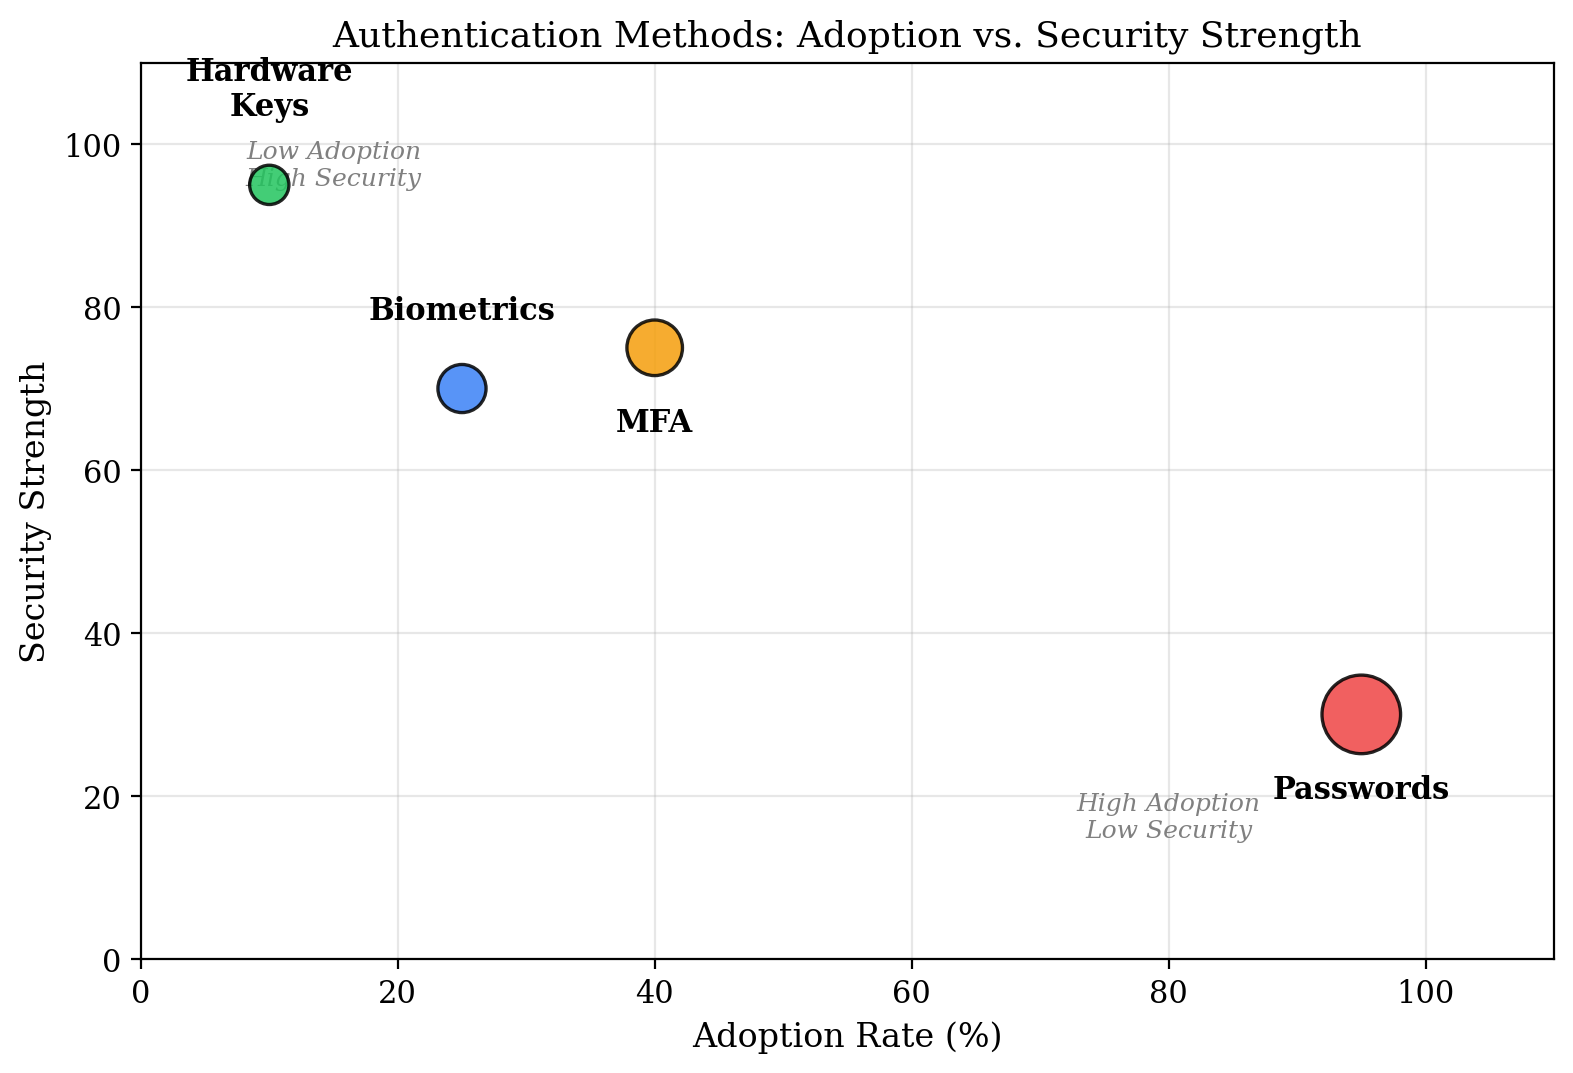
\includegraphics[width=0.85\textwidth]{figures/auth_methods_comparison.png}
    \caption{Comparison of authentication methods by adoption rate and security strength.}
    \label{fig:auth_methods}
\end{figure}

Therefore, improving password quality is still a crucial part of cybersecurity. This includes encouraging users to create strong, unique passwords and designing systems, such as the proposed password strength evaluation tool, that help users and administrators better understand and reduce the risks associated with weak passwords.

\section{Common Password Vulnerabilities}

During my research, I identified several factors that contribute to weak passwords. Table~\ref{tab:vulnerability_examples} summarises the most common vulnerability types, provides concrete examples, and links each to its impact on the password search space and the attack methods that exploit it.

\begin{table}[H]
\centering
\caption{Common password vulnerability types, examples, and their security impact.}
\label{tab:vulnerability_examples}
\begin{tabularx}{\textwidth}{>{\raggedright\arraybackslash}p{2.8cm} >{\raggedright\arraybackslash}p{2.5cm} >{\raggedright\arraybackslash}p{3cm} >{\raggedright\arraybackslash}p{3.5cm}}
\toprule
\textbf{Vulnerability Type} & \textbf{Example} & \textbf{Search Space Impact} & \textbf{Attack Method} \\
\midrule
Short length & \texttt{abc1} & $26^{4} \approx 457{,}000$ combinations & Brute-force (seconds) \\
\midrule
Lack of complexity & \texttt{password} & $26^{8} \approx 2 \times 10^{11}$ vs.\ $94^{8} \approx 6 \times 10^{15}$ & Dictionary attack \\
\midrule
Reused passwords & Same password on 5+ sites & One breach compromises all accounts & Credential stuffing \\
\midrule
Dictionary words & \texttt{sunshine2024} & Predictable structure: word + year & Dictionary with mutation rules \\
\midrule
Personal information & \texttt{John1995!} & Guessable via social engineering & Targeted dictionary attack \\
\bottomrule
\end{tabularx}
\end{table}

\begin{figure}[H]
    \centering
    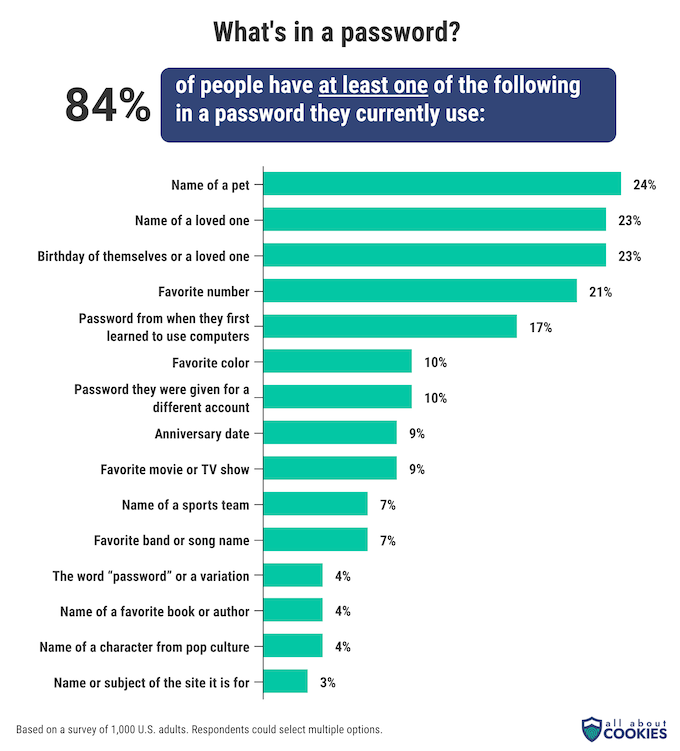
\includegraphics[width=0.85\textwidth]{figures/password_behaviour.png}
    \caption{User dangerous password behaviours.}
    \label{fig:password_behaviour}
\end{figure}

The fundamental problem with each of these vulnerabilities is that they reduce the effective search space an attacker must explore. A password that appears long and complex but follows a predictable pattern (such as a dictionary word with appended digits) can often be cracked faster than a shorter but truly random string, because attackers optimise their strategies by trying the most likely patterns first \cite{weir2009}.


\section{Mechanisms of Password Attacks}

Understanding how attackers attempt to compromise passwords is essential for designing effective evaluation criteria. This section describes the four principal categories of password attacks and explains how each motivates a specific dimension of the evaluation algorithm developed in this thesis.

\subsection{Brute-Force Attacks}

In a brute-force attack, the attacker systematically tries every possible combination of characters until the correct password is found. For a password of length $L$ drawn from a character set of size $N$, the total number of possible combinations is $N^{L}$. Modern hardware, particularly graphics processing units (GPUs), can attempt billions of guesses per second, making short passwords with small character sets trivially breakable.

\begin{figure}[H]
    \centering
    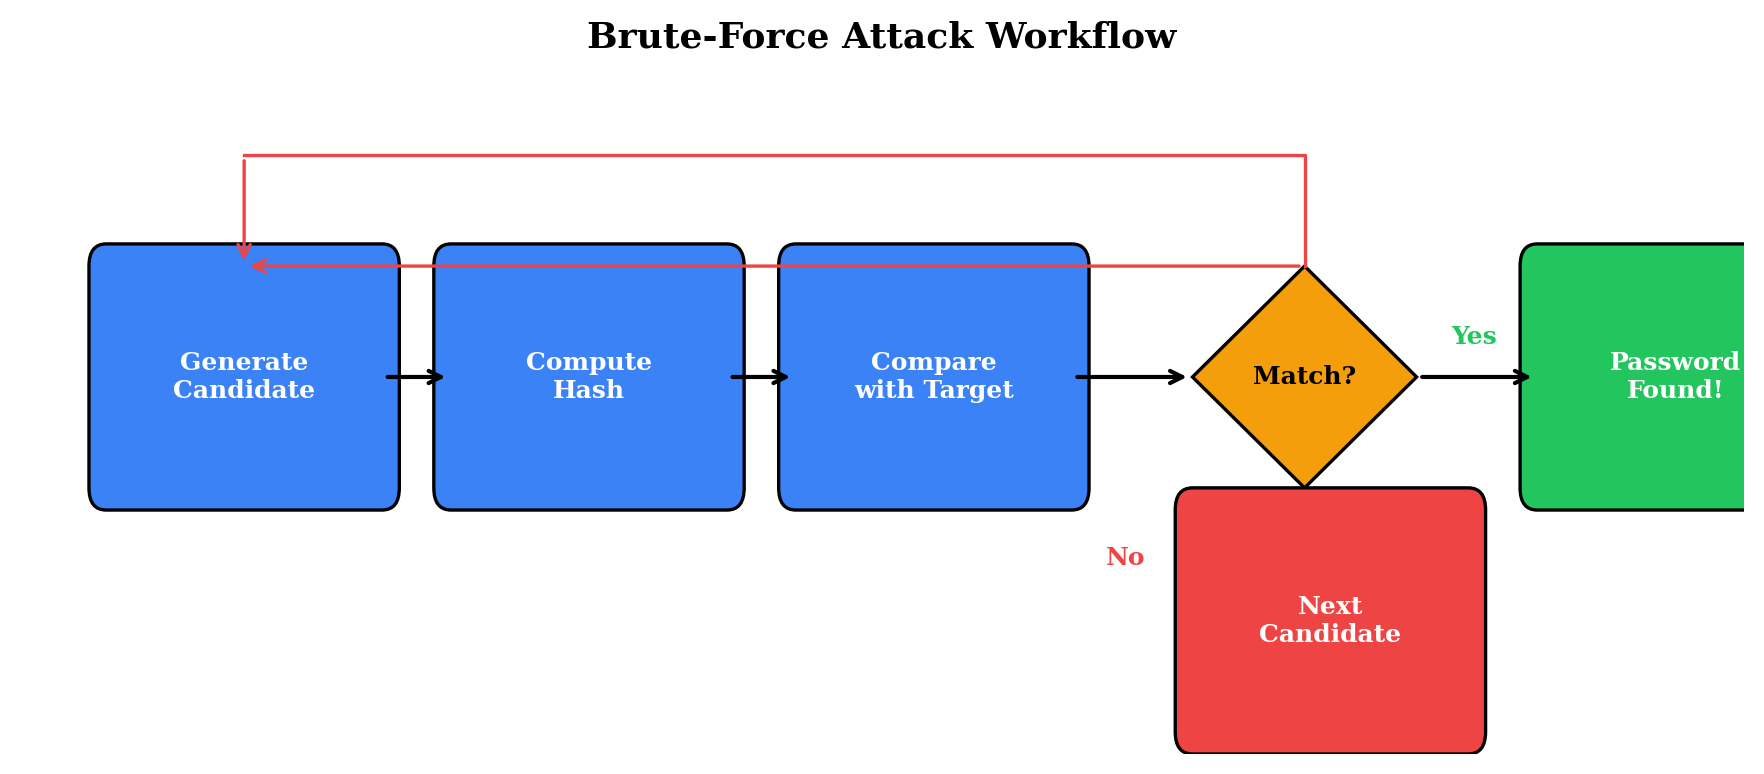
\includegraphics[width=0.85\textwidth]{figures/brute_force_workflow.png}
    \caption{Workflow of a brute-force attack.}
    \label{fig:brute_force}
\end{figure}

The time required for a brute-force attack grows exponentially with password length. This exponential relationship is the primary motivation for the length scoring dimension in the evaluation algorithm: longer passwords receive higher scores because they are exponentially harder to crack by exhaustive search.

\subsection{Dictionary Attacks}

A dictionary attack improves upon brute-force by using a pre-compiled list of likely passwords (a ``dictionary'') rather than trying every possible combination. The dictionary typically contains common passwords, words from natural language, and known leaked credentials. More sophisticated dictionary attacks apply mutation rules to each dictionary entry---capitalising the first letter, appending digits, replacing letters with similar-looking symbols (leetspeak), and combining multiple words.

\begin{figure}[H]
    \centering
    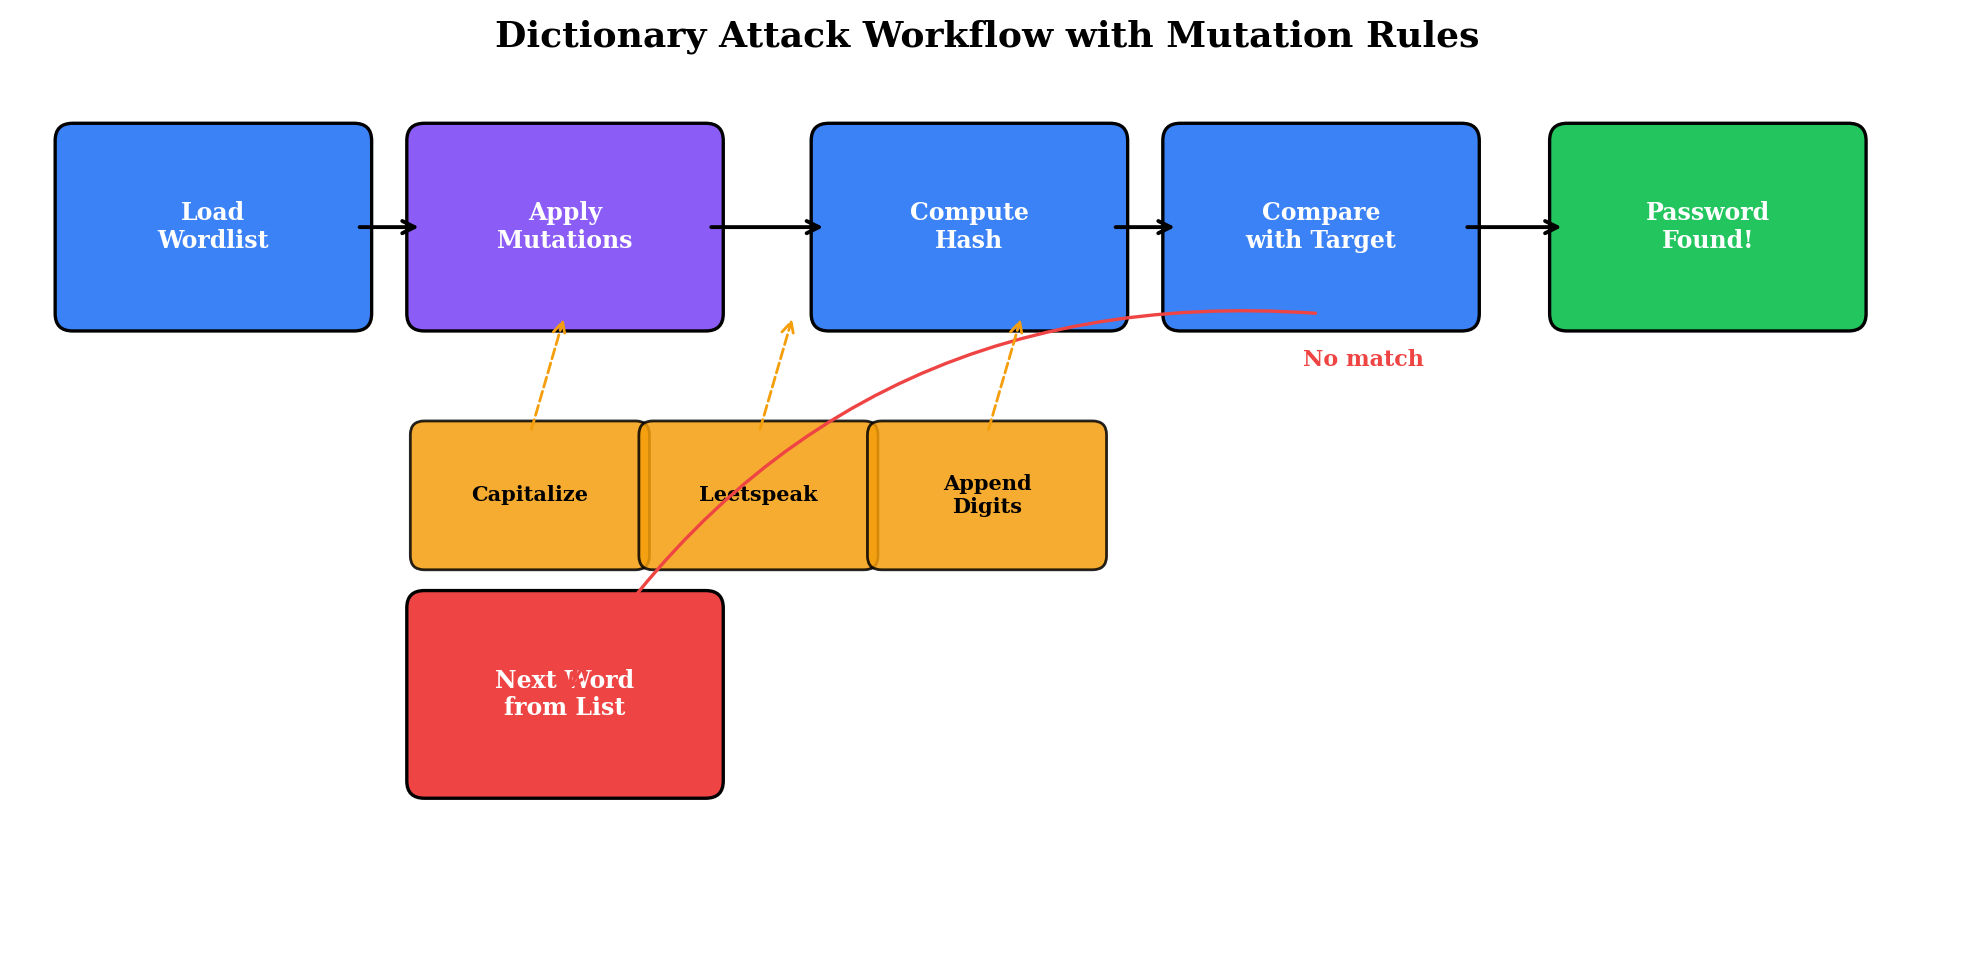
\includegraphics[width=0.85\textwidth]{figures/dictionary_attack_workflow.png}
    \caption{Workflow of a dictionary attack with common mutation rules.}
    \label{fig:dictionary_attack}
\end{figure}

Dictionary attacks are highly effective because most users choose passwords that follow predictable patterns. Wheeler demonstrated that the zxcvbn strength estimator, which models common password patterns, can crack many supposedly ``strong'' passwords far more efficiently than brute-force alone \cite{wheeler2016}. This motivates the dictionary comparison and Levenshtein similarity dimensions in the evaluation algorithm.

\subsection{Credential Stuffing}

Credential stuffing is an attack in which usernames and password pairs leaked from one breach are systematically tested against other online services. The attack exploits the widespread practice of password reuse: if a user employs the same password on multiple sites, a single breach compromises all of their accounts.

\begin{figure}[H]
    \centering
    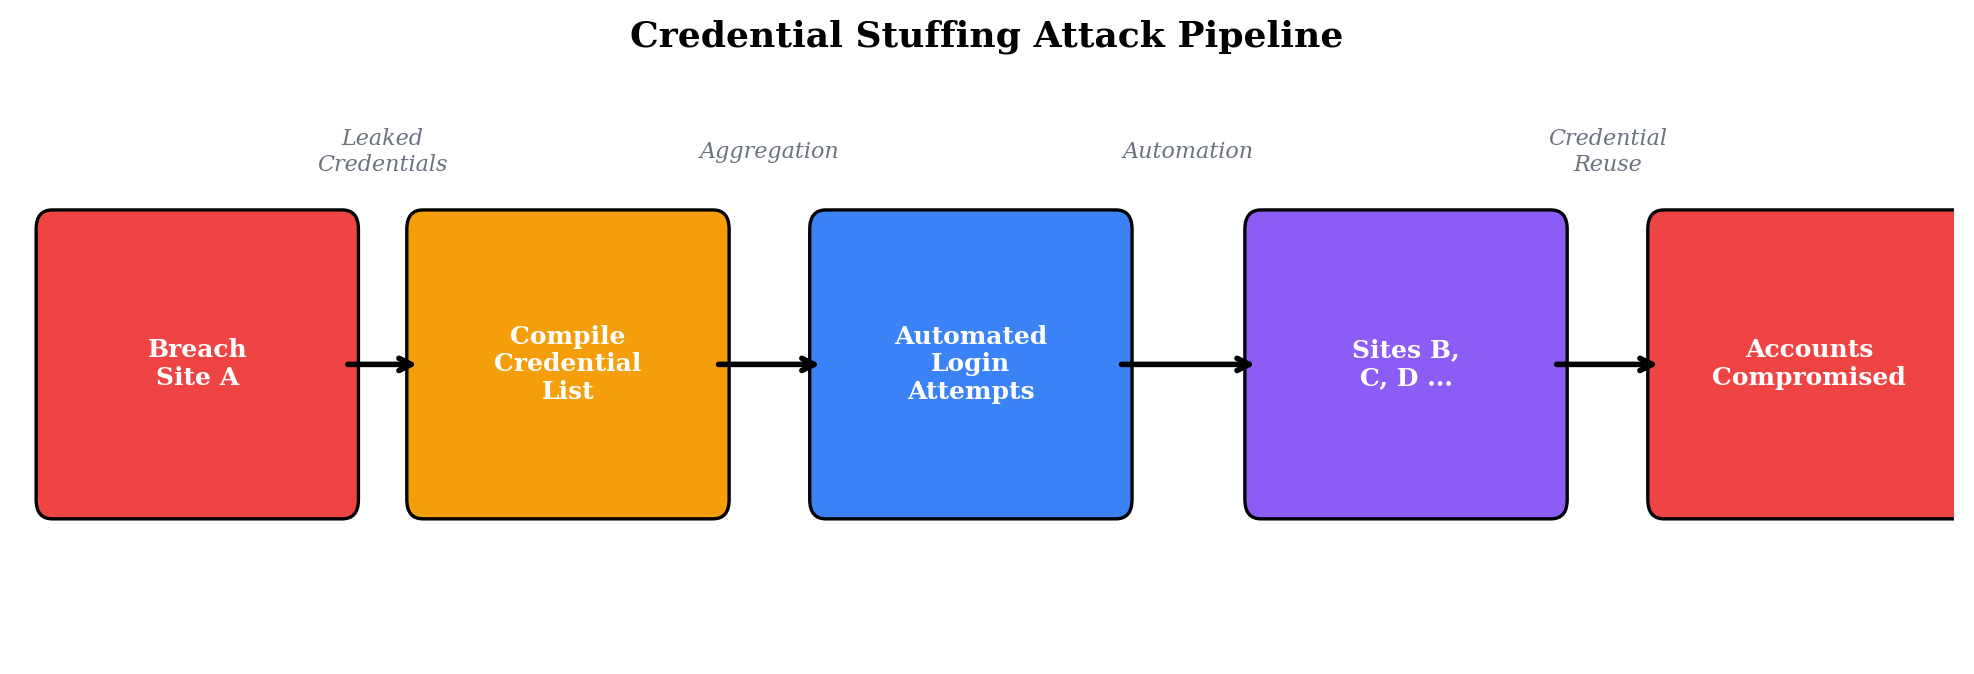
\includegraphics[width=0.85\textwidth]{figures/credential_stuffing_pipeline.png}
    \caption{Pipeline of a credential stuffing attack.}
    \label{fig:credential_stuffing}
\end{figure}

Credential stuffing attacks have been implicated in numerous high-profile incidents, including the Zoom breach of 2020, where attackers used credentials leaked from earlier breaches to access Zoom accounts \cite{verizon2024}. While the evaluation tool cannot directly prevent credential stuffing (which is a behavioural issue rather than a technical one), it can encourage users to create unique passwords by highlighting the risks of common and reused credentials.

\subsection{Rainbow Table Attacks}

Rainbow tables are pre-computed lookup tables that map cryptographic hash values to their corresponding plaintext passwords. Instead of computing the hash for each candidate password during an attack, the attacker simply looks up the stolen hash in the rainbow table. This approach trades storage space for computation time and is extremely efficient against unsalted password hashes.

Modern systems mitigate rainbow table attacks by using salted hashes (appending a random value to each password before hashing), which renders pre-computed tables useless. However, rainbow tables remain relevant for legacy systems that store unsalted hashes, and their existence underscores the importance of ensuring that even if a hash is stolen, the underlying password should be sufficiently complex to resist all attack methods.

\clearpage

\section{Real-World Examples of Password Breaches}

I also reviewed notable cybersecurity incidents that demonstrated the consequences of weak passwords and poor credential management:

\begin{itemize}
    \item \textbf{LinkedIn (2012):} Over 117 million passwords were leaked due to inadequate password hashing and users choosing simple combinations like ``123456.''\\
    The LinkedIn breach highlighted not only weak user passwords but also the risks of inadequate hashing mechanisms, allowing attackers to recover millions of credentials efficiently.

    \item \textbf{Facebook (2019):} Hundreds of millions of user passwords were stored in plaintext and accidentally logged in internal systems accessible to thousands of employees. While there was no confirmed large-scale external leak, it exposed how poor internal password handling can create serious insider and data exposure risks.\\
    This incident showed that strong user passwords are not sufficient on their own; organisations must also enforce secure storage practices (e.g., salted hashing) and strict access controls to prevent exposure from misconfigurations and internal tooling.

    \item \textbf{Zoom (2020):} During the early COVID-19 pandemic, attackers used ``credential stuffing'' with passwords leaked from older breaches to break into Zoom accounts and meetings, taking advantage of users who reused passwords across services.\\
    The Zoom incidents demonstrated how password reuse turns one breach into many, emphasising the need for unique passwords per site and support for multi-factor authentication to limit the impact of credential stuffing.

    \item \textbf{Colonial Pipeline (2021):} Ransomware operators accessed a VPN account using a compromised password that was found in a previous data breach and reportedly not protected by multi-factor authentication. The attack disrupted fuel supply across the U.S.\ East Coast.\\
    This case illustrated how a single exposed and reused password, combined with a lack of MFA on remote access, can have real-world physical and economic consequences far beyond the IT environment.

    \item \textbf{NVIDIA (2022):} An attacker group claimed to have accessed internal systems and leaked employee credentials and certificates. Password reuse and weak internal credential practices were reported as contributing factors, enabling deeper access once an initial foothold was gained.\\
    The NVIDIA incident underscored how weak or reused internal passwords can allow lateral movement inside corporate networks, turning one compromised account into widespread access to sensitive intellectual property.

    \item \textbf{LastPass (2022--2023):} An engineer's home machine was compromised, and an account protected by a master password was targeted. While the immediate cause was not a simple weak password list, the incident reignited concerns about master passwords, password vault security, and user password hygiene for the vault itself.\\
    The LastPass breach highlighted that even when password managers are used, the strength of the master password (and additional factors like MFA and device security) is critical, since compromising a single high-value credential can expose many others.

    \item \textbf{MOVEit-related credential attacks (2023):} In parallel with exploiting MOVEit vulnerabilities, threat actors also attempted to use previously leaked or weak credentials to access related infrastructure and accounts, combining software flaws with poor password practices.\\
    These campaigns showed how attackers increasingly blend vulnerability exploitation with credential-based attacks, meaning weak or reused passwords make organisations far more vulnerable even when patching cycles improve.
\end{itemize}

These examples reinforce the need for stronger user education, unique and complex passwords, multi-factor authentication, and secure organisational handling of credentials---which is precisely what I aimed to address through my project.


\section{Password Strength Evaluation Methods}

While studying password security, I came across several common methods used to measure password strength:

\begin{itemize}
    \item \textbf{Rule-based analysis:} Evaluates whether a password meets specific conditions (e.g., minimum length, inclusion of uppercase letters, numbers, and symbols). This approach is simple and transparent but often fails to capture deeper weaknesses such as dictionary words or predictable patterns.
    \item \textbf{Entropy-based analysis:} Estimates password unpredictability using information theory \cite{shannon1948}. Higher entropy values usually mean stronger passwords, but entropy alone does not account for patterns or dictionary words that may be tried first by attackers.
    \item \textbf{Dictionary comparison:} Checks if a password appears in known leaked datasets or common password lists. This method directly addresses the most likely attack strategy but does not evaluate structural properties like length or diversity.
    \item \textbf{Machine learning approaches:} More advanced models attempt to predict password strength using neural networks trained on large datasets \cite{melcher2016, castelluccia2012}. While effective, they are more complex to implement and operate as ``black boxes,'' making it difficult to explain the reasoning behind a particular strength rating.
\end{itemize}

For my project, I decided to combine the first three methods---rule-based checks, entropy calculation, and dictionary comparison---into a hybrid evaluation algorithm that balances simplicity, accuracy, and transparency. The hybrid approach addresses a key limitation of each individual method: rule-based checks miss patterns, entropy misses dictionary words, and dictionary checks miss structural weaknesses. By combining all three, the tool provides a more comprehensive assessment.


\section{Entropy and Password Strength}

Entropy represents the amount of unpredictability or randomness in a password. In information theory, it is measured in bits using the following formula, as introduced by Shannon \cite{shannon1948}:

\begin{equation}
H = L \times \log_2 N
\end{equation}

where $L$ is the password length and $N$ is the number of possible characters per position (for example, 26 for lowercase letters, 10 for digits, etc.). Higher entropy values correspond to more secure passwords.

\textbf{Intuitive explanation of log₂ and bits:}
The logarithm base 2 (log₂) measures how many times you need to double 1 to reach a value, or equivalently, how many binary decisions (bits) are needed to represent a number. Each bit of entropy represents a doubling of the guess space required to crack the password via brute-force.
\begin{itemize}
    \item 1 bit = 2 possibilities (0 or 1) -- requires 1 guess on average to crack
    \item 2 bits = 4 possibilities (00, 01, 10, 11) -- requires 2 guesses on average
    \item 10 bits = 1,024 possibilities -- requires 512 guesses on average
    \item 20 bits = 1,048,576 possibilities -- requires 524,288 guesses on average
    \item 30 bits = 1,073,741,824 possibilities -- requires 536,870,912 guesses on average
    \item 40 bits = 1 trillion possibilities -- requires 500 billion guesses on average
\end{itemize}
For example, an 8-character password using only lowercase letters has approximately:

\begin{equation}
H = 8 \times \log_2 26 \approx 37.6 \text{ bits}
\end{equation}

This means an attacker would need to try, on average, 2³⁷·⁶/2 ≈ 2³⁶·⁶ ≈ 100 billion guesses to crack it via brute-force.

While a password including uppercase letters, digits, and symbols could exceed 60 bits---offering much stronger protection against brute-force attacks.

Table~\ref{tab:entropy_charset} provides a comprehensive comparison of entropy values across different password lengths and character set compositions, illustrating how both length and character diversity contribute to password strength.

\begin{table}[H]
\centering
\caption{Password entropy (bits) by length and character set composition.}
\label{tab:entropy_charset}
\begin{tabularx}{\textwidth}{ccccc}
\toprule
\textbf{Length} & \textbf{Lowercase only} & \textbf{+ Uppercase} & \textbf{+ Digits} & \textbf{+ Symbols} \\
 & ($N = 26$) & ($N = 52$) & ($N = 62$) & ($N = 94$) \\
\midrule
6  & 28.2  & 34.3  & 35.6  & 39.3  \\
8  & 37.6  & 45.7  & 47.5  & 52.4  \\
10 & 47.0  & 57.2  & 59.4  & 65.5  \\
12 & 56.4  & 68.6  & 71.3  & 78.6  \\
16 & 75.2  & 91.5  & 95.1  & 104.8 \\
\bottomrule
\end{tabularx}
\end{table}

The table clearly demonstrates that both length and character set diversity independently contribute to entropy, and that their combined effect is multiplicative. A 12-character password using all four character categories (78.6 bits) is roughly $2^{26}$ (approximately 67 million) times harder to crack by brute-force than a 12-character lowercase-only password (56.4 bits).

\begin{figure}[H]
    \centering
    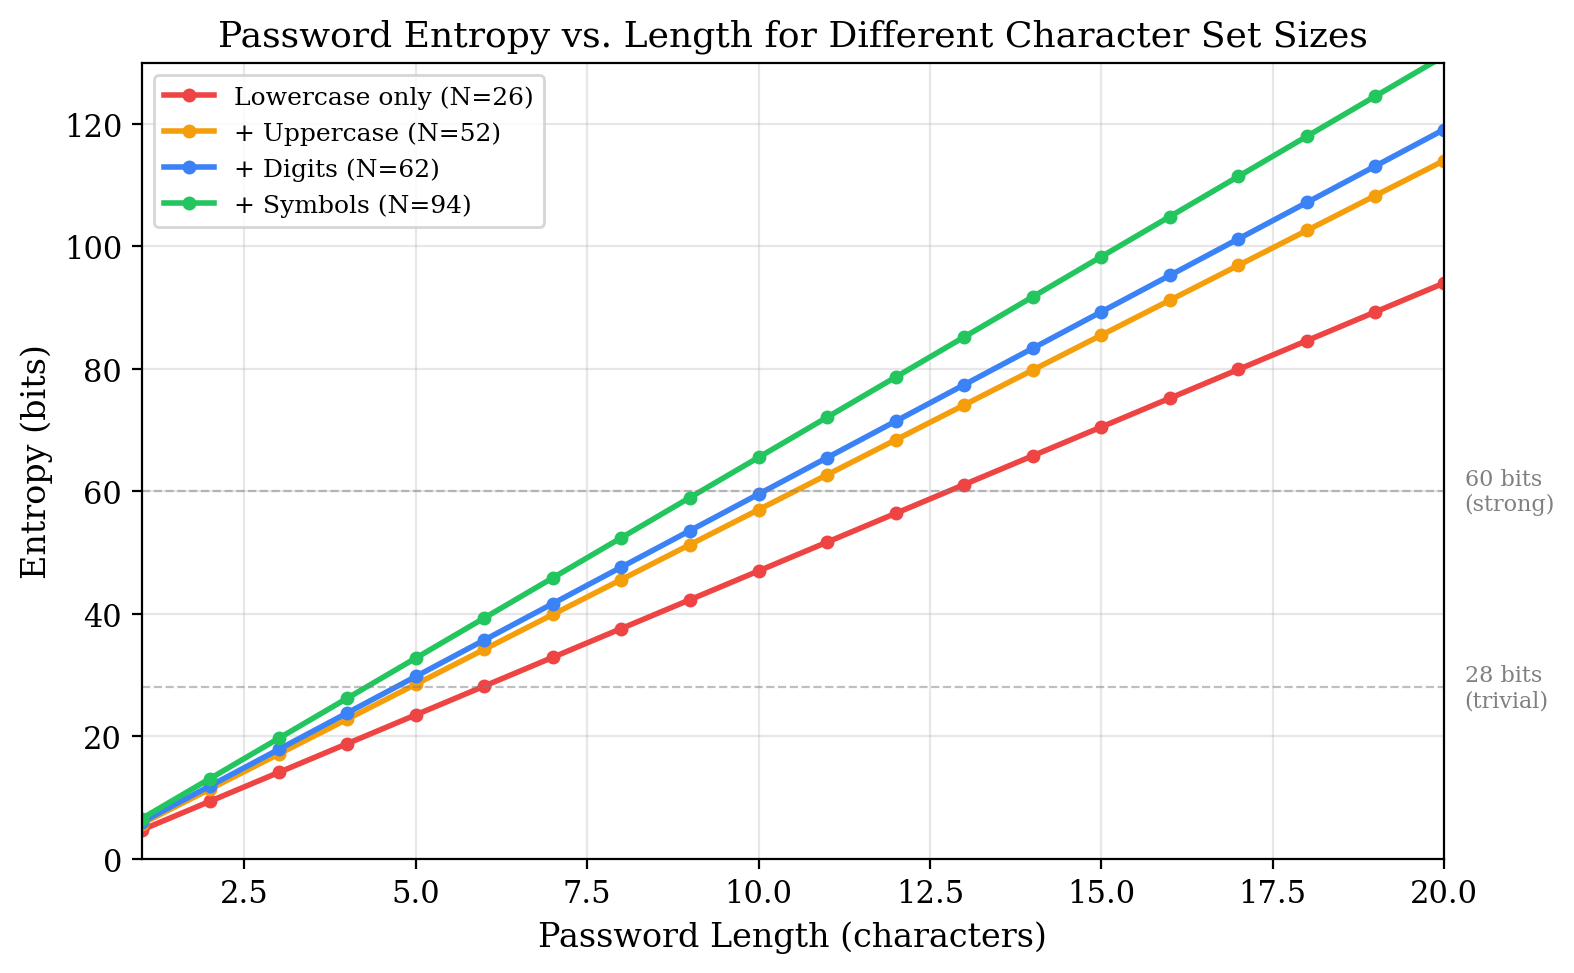
\includegraphics[width=0.85\textwidth]{figures/entropy_vs_length_graph.png}
    \caption{Entropy as a function of password length for four character set compositions.}
    \label{fig:entropy_graph}
\end{figure}

Consider a concrete comparison: the password \texttt{abcdefgh} (8 lowercase characters) has an entropy of approximately 37.6 bits, while the password \texttt{aB1!xY9\#} (8 characters mixing all categories) has an entropy of approximately 52.4 bits. Despite having the same length, the mixed-charset password is roughly $2^{14.8} \approx 28{,}000$ times harder to crack by brute-force. This example illustrates why both length and diversity are essential dimensions in a password strength evaluation model.

\textbf{Worked crack time examples:}
Assuming an attacker capable of 10¹⁰ guesses per second (10 billion/second, realistic for modern GPU cracking):
\begin{itemize}
    \item \texttt{abcdefgh} (37.6 bits): Average crack time = 2³⁷·⁶ / 2×10¹⁰ ≈ 100 billion ÷ 20 billion = 5 seconds
    \item \texttt{aB1!xY9\#} (52.4 bits): Average crack time = 2⁵²·⁴ / 2×10¹⁰ ≈ 4.5 million billion ÷ 20 billion ≈ 225,000 seconds ≈ 2.6 days
    \item \texttt{TestPass123!} (72.1 bits): Average crack time = 2⁷²·¹ / 2×10¹⁰ ≈ 50 billion billion ÷ 20 billion ≈ 2.5 billion seconds ≈ 79 years
    \item Generated 16-char password (104.8 bits): Average crack time = 2¹⁰⁴·⁸ / 2×10¹⁰ ≈ 20,000 billion billion billion ÷ 20 billion ≈ 18,000 centuries
\end{itemize}
This shows why entropy alone doesn't determine practical security---a password like \texttt{password} (which would have 37.6 bits if truly random) falls instantly to dictionary attacks despite the brute-force estimate of 5 seconds.


\section{Existing Tools and Standards}

Several password checkers and guidelines influenced my approach. Table~\ref{tab:tools_comparison} presents a formal comparison of the most relevant tools and standards.

\begin{table}[H]
\centering
\caption{Comparison of password strength evaluation tools and standards.}
\label{tab:tools_comparison}
\begin{tabularx}{\textwidth}{lcccc}
\toprule
\textbf{Tool / Standard} & \textbf{Method} & \textbf{Online / Offline} & \textbf{Breach Database} & \textbf{Open Source} \\
\midrule
Our tool & Hybrid (rules + entropy + patterns + dictionary) & Offline & Local list (181 entries) & Yes \\
zxcvbn \cite{wheeler2016} & Pattern matching + entropy & Offline & Built-in frequency list & Yes \\
Have I Been Pwned \cite{hibp2021} & Breach database lookup & Online & 600M+ entries & Partially \\
NordPass Checker \cite{nordpass2024} & Rule-based + breach data & Online & Proprietary & No \\
NIST SP 800-63B \cite{nist2017} & Guidelines (blacklist-based) & N/A & Recommends breach check & N/A \\
\bottomrule
\end{tabularx}
\end{table}

The \textbf{NIST Digital Identity Guidelines (SP 800-63B)}, published in 2017 and updated in 2020, represent a significant shift in password policy philosophy \cite{nist2017}. The guidelines recommend:

\begin{itemize}
    \item Avoiding arbitrary composition rules (e.g., ``must contain at least one uppercase letter and one digit'') that lead to predictable patterns,
    \item Using blacklist-based validation, checking passwords against known compromised password lists,
    \item Allowing all printable ASCII characters and Unicode characters,
    \item Permitting paste functionality to support password managers,
    \item Not requiring periodic password changes unless there is evidence of compromise.
\end{itemize}

\begin{figure}[H]
    \centering
    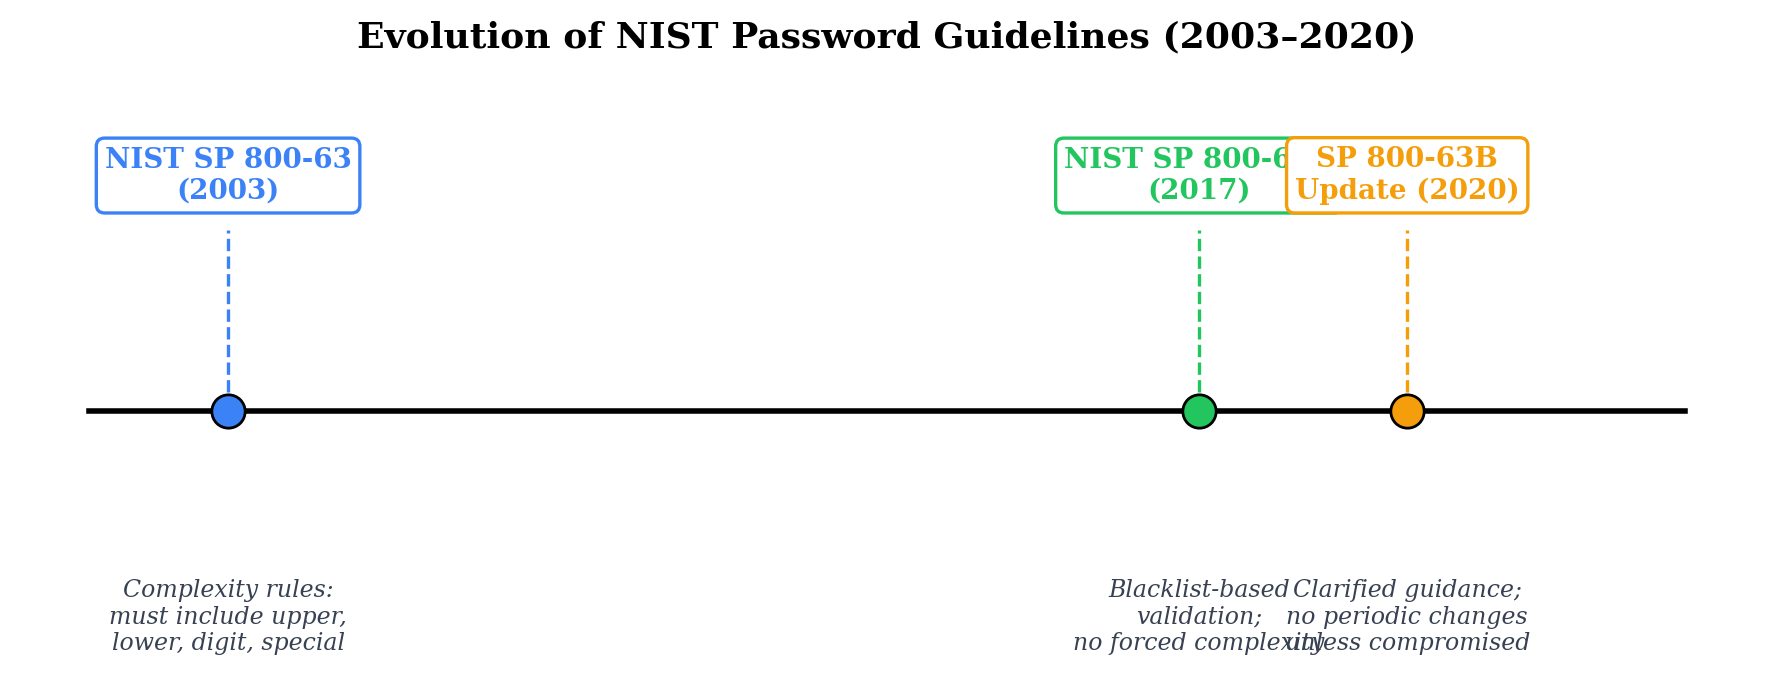
\includegraphics[width=0.85\textwidth]{figures/nist_guidelines_timeline.png}
    \caption{Evolution of NIST password guidelines from complexity rules to blacklist-based validation.}
    \label{fig:nist_timeline}
\end{figure}

By analyzing these existing tools and standards, I learned that effective password evaluation should combine mathematical rigor with user-friendly feedback — a balance I aimed to achieve in my own implementation. The NIST guidelines, in particular, motivated my decision to include dictionary comparison and to keep the scoring model transparent through named constants, so that users can understand why a particular score was assigned rather than relying on a ``black box'' assessment.


\section{Summary}

In this chapter, I reviewed the theoretical foundations of password security and evaluation. I discussed the role of passwords in modern authentication, identified common vulnerability types and their security impact, described the mechanisms of the four principal categories of password attacks, examined real-world breach examples, reviewed the four main approaches to password strength evaluation, provided a detailed analysis of entropy and its relationship to password strength, and compared existing tools and standards.

The key insight from this review is that no single evaluation method is sufficient on its own: rule-based checks miss patterns, entropy misses dictionary words, and dictionary checks miss structural weaknesses. This motivates the hybrid approach adopted in this thesis, which combines all three methods into a single, transparent scoring model. The next chapter describes the methodology used to implement this hybrid approach.

%=============================================================================
% CHAPTER 3: METHODOLOGY
%=============================================================================
\chapter{Methodology}

\section{Overview}

In this chapter, I describe the methodology I followed to transform the theoretical background into a practical, functional password strength evaluation tool. My approach was iterative: I started by analysing requirements, then designed a modular architecture, implemented the core logic in Python, and systematically improved the tool through 18 enhancements and a user-experience redesign. Throughout this process, I focused on modularity, usability, and user privacy.

The iterative development process followed this general pattern: (1) define requirements and design the architecture, (2) implement the initial version of each module, (3) test the tool with representative passwords and identify weaknesses, (4) implement targeted improvements, and (5) repeat from step 3 until the tool met the desired quality standards. This process resulted in 18 documented enhancements covering scoring accuracy, pattern detection coverage, dictionary comparison, user interface improvements, and overall code quality. A subsequent user-experience redesign restructured the interface from a basic layout to a two-column analysis dashboard with animated visual indicators.

\clearpage

\section{System Requirements and Technology Justification}

The tool was developed to run as a desktop application on the Windows operating system. The technical requirements are as follows:

\begin{itemize}
    \item \textbf{Programming language:} Python 3.14, selected for its readability, strong string manipulation capabilities, extensive standard library, and support for modern type annotations.
    \item \textbf{GUI framework:} CustomTkinter (version 5.2.0 or later), a modern wrapper around Tkinter that provides native-looking dark-themed widgets with minimal configuration.
    \item \textbf{Platform:} Windows desktop. The application creates a fixed-size, non-resizable window (1000$\times$780 pixels) centred on the screen.
    \item \textbf{Network:} No network connection is required. All processing happens locally, and no passwords are stored, logged, or transmitted at any point.
    \item \textbf{Hardware assumptions for crack time estimation:} The tool assumes an attacker capable of 10 billion guesses per second, consistent with modern GPU-based cracking rigs.
\end{itemize}

The only external dependency beyond the Python standard library is CustomTkinter. All other modules---\texttt{math}, \texttt{re}, \texttt{secrets}, \texttt{string}, \texttt{os}, \texttt{sys}, \texttt{dataclasses}---are part of the Python standard library, minimising installation complexity and reducing the attack surface of the application.

\subsection{Why Python}

Python was chosen as the programming language for this project for several compelling reasons:

\begin{itemize}
    \item \textbf{Readability and maintainability:} Python's syntax emphasises clarity and uses indentation to define code blocks, resulting in code that is easy to read, review, and maintain. For a thesis project that must be understood and evaluated by others, this readability is a significant advantage over more verbose languages such as Java or C++.

    \item \textbf{Rapid development:} Python's dynamic typing, interactive interpreter, and concise syntax allow features to be prototyped and tested quickly. This was particularly valuable during the iterative development process, where 18 enhancements and a UX redesign were implemented in rapid succession.

    \item \textbf{Strong standard library:} Python's standard library provides built-in modules for regular expressions (\texttt{re}), mathematical operations (\texttt{math}), cryptographic random number generation (\texttt{secrets}), string manipulation (\texttt{string}), and immutable data structures (\texttt{dataclasses}). These modules eliminated the need for external dependencies for all core evaluation logic.

    \item \textbf{String manipulation ergonomics:} Password evaluation is fundamentally a string-analysis task. Python's first-class Unicode support, slicing syntax, list comprehensions, and generator expressions make string processing operations concise and expressive. A pattern detection function that requires 20 lines in Python might require 40--60 lines in Java or C++ due to the absence of these conveniences.

    \item \textbf{Type annotations:} Python 3.14 supports modern type annotations (e.g., \texttt{list[str]}, \texttt{dict[str, bool]}, \texttt{str | None}), which improve code documentation and enable static type checking with tools like \texttt{mypy}. The \texttt{EvaluationResult} dataclass uses typed fields, making the API contract explicit and self-documenting.

    \item \textbf{Portability and cross-platform capability:} While the current implementation targets Windows, Python runs on all major operating systems. The evaluation engine (evaluator, entropy, patterns, dictionary\_check) has no platform-specific code and could be used on Linux or macOS without modification. Only the GUI module would need minor adjustments for platform-specific font rendering.
\end{itemize}

\textbf{Why not alternative languages?} Java was considered but rejected due to its verbosity (boilerplate class definitions, explicit type declarations, and getter/setter patterns) and its lack of concise string processing syntax. C++ was rejected because manual memory management and pointer arithmetic add unnecessary complexity for a string-processing application with no performance-critical bottlenecks. JavaScript was rejected because browser-based tools raise privacy concerns---the password must be processed client-side with no server transmission, which is harder to guarantee in a web environment where network requests can be made invisibly. Python's local-only execution model provides a stronger guarantee of privacy by default.

\subsection{Library-by-Library Justification}

Each module and library used in the project was selected for a specific reason:

\begin{itemize}
    \item \textbf{\texttt{re} (regular expressions):} Used for character classification in the entropy module. Pre-compiled regex patterns (\texttt{\_RE\_LOWER}, \texttt{\_RE\_UPPER}, \texttt{\_RE\_DIGIT}, \texttt{\_RE\_SPECIAL}) efficiently determine which character categories appear in the password. Pre-compilation avoids the overhead of recompiling the same patterns on every call, which is important because \texttt{classify\_characters()} may be called multiple times per evaluation (once for entropy and once for diversity scoring).

    \item \textbf{\texttt{math} (mathematical functions):} Used for the $\log_2$ computation in the entropy formula $H = L \times \log_2 N$. Python's \texttt{math.log2()} function provides high-precision floating-point results, which is essential for accurate entropy estimation and crack time calculation.

    \item \textbf{\texttt{secrets} (cryptographic random number generation):} Used exclusively for password generation. The \texttt{secrets} module draws from the operating system's cryptographically secure random number generator (e.g., \texttt{CryptGenRandom} on Windows, \texttt{/dev/urandom} on Linux), unlike the \texttt{random} module's Mersenne Twister algorithm, which is statistically adequate but not cryptographically secure. The decision to use \texttt{secrets.choice()} for character selection and \texttt{secrets.SystemRandom().shuffle()} for randomisation ensures that generated passwords cannot be predicted even if an attacker knows the internal state of the random number generator.

    \item \textbf{\texttt{dataclasses} (structured data):} Used to define the \texttt{EvaluationResult} dataclass with \texttt{frozen=True}, which creates an immutable, typed, and self-documenting result object. The immutability guarantee prevents accidental modification of results after creation, and the automatic generation of \texttt{\_\_init\_\_}, \texttt{\_\_repr\_\_}, and \texttt{\_\_eq\_\_} methods reduces boilerplate code. The dataclass also includes per-dimension score breakdown fields (\texttt{length\_pts}, \texttt{diversity\_pts}, \texttt{entropy\_pts}, \texttt{pattern\_pts}, \texttt{dict\_pts}), enabling the GUI to display a detailed breakdown of how each dimension contributed to the final score.

    \item \textbf{\texttt{frozenset} (immutable set for O(1) membership testing):} Used in the pattern detection module to define \texttt{\_ASCII\_LOWER}, \texttt{\_ASCII\_UPPER}, and \texttt{\_ASCII\_DIGIT} as immutable sets. The use of \texttt{frozenset} rather than \texttt{set} makes the intent clear (these collections never change) and provides $O(1)$ average-case membership testing for the character filtering step in \texttt{detect\_sequential()}, which is called on every evaluation.

    \item \textbf{CustomTkinter (GUI framework):} Selected over several alternatives for the graphical interface:
    \begin{itemize}
        \item \textbf{Over plain \texttt{tkinter}:} Standard Tkinter provides basic widgets but lacks modern styling (dark themes, rounded corners, smooth animations). CustomTkinter wraps Tkinter with a modern aesthetic while retaining its simplicity and cross-platform compatibility.
        \item \textbf{Over PyQt / PySide:} The Qt framework is powerful but introduces a large external dependency (30+ MB), a complex licensing model (GPL vs.\ LGPL vs.\ commercial), and a steeper learning curve. For a focused thesis project, the additional capability is unnecessary.
        \item \textbf{Over Kivy:} Kivy targets mobile and touch interfaces, which is not the deployment target. Its custom rendering engine also produces a non-native look and feel on desktop platforms.
    \end{itemize}
    CustomTkinter provides the ideal balance: a single lightweight dependency, native-looking dark-themed widgets, and full access to the underlying Tkinter canvas for custom drawing (the semicircular gauge).
\end{itemize}


\section{Architecture}

The tool is structured as a Python package called \texttt{password\_tool} containing five core modules, each with a distinct responsibility. This modular design ensures separation of concerns: the evaluation logic is entirely independent of the graphical interface and can be tested and used in isolation.

\begin{itemize}
    \item \textbf{main.py} --- Graphical user interface. Defines the \texttt{PasswordAnalyzerApp} class, which creates the CustomTkinter window, handles user input, and displays evaluation results. This module is the only one that depends on CustomTkinter.
    \item \textbf{evaluator.py} --- Scoring engine. Combines the five analysis dimensions into a single 0--100 score and returns an immutable \texttt{EvaluationResult} dataclass. Also contains the \texttt{generate\_password} function.
    \item \textbf{entropy.py} --- Entropy calculation. Implements Shannon entropy estimation, character classification, entropy-to-score mapping, and brute-force crack time estimation.
    \item \textbf{patterns.py} --- Pattern detection. Detects sequential characters, repeated characters, and keyboard-row patterns (including reversed variants).
    \item \textbf{dictionary\_check.py} --- Dictionary comparison. Provides exact match, substring detection, and Levenshtein distance similarity checking against a common-passwords list.
\end{itemize}

Supporting files include \texttt{\_\_init\_\_.py} (marks the directory as a Python package), \texttt{\_\_main\_\_.py} (entry point for \texttt{python -m password\_tool}), and \texttt{common\_passwords.txt} (a curated list of 181 common and leaked passwords). The external files \texttt{requirements.txt} and \texttt{run.bat} manage dependencies and provide a convenient Windows launcher.

\begin{figure}[H]
    \centering
    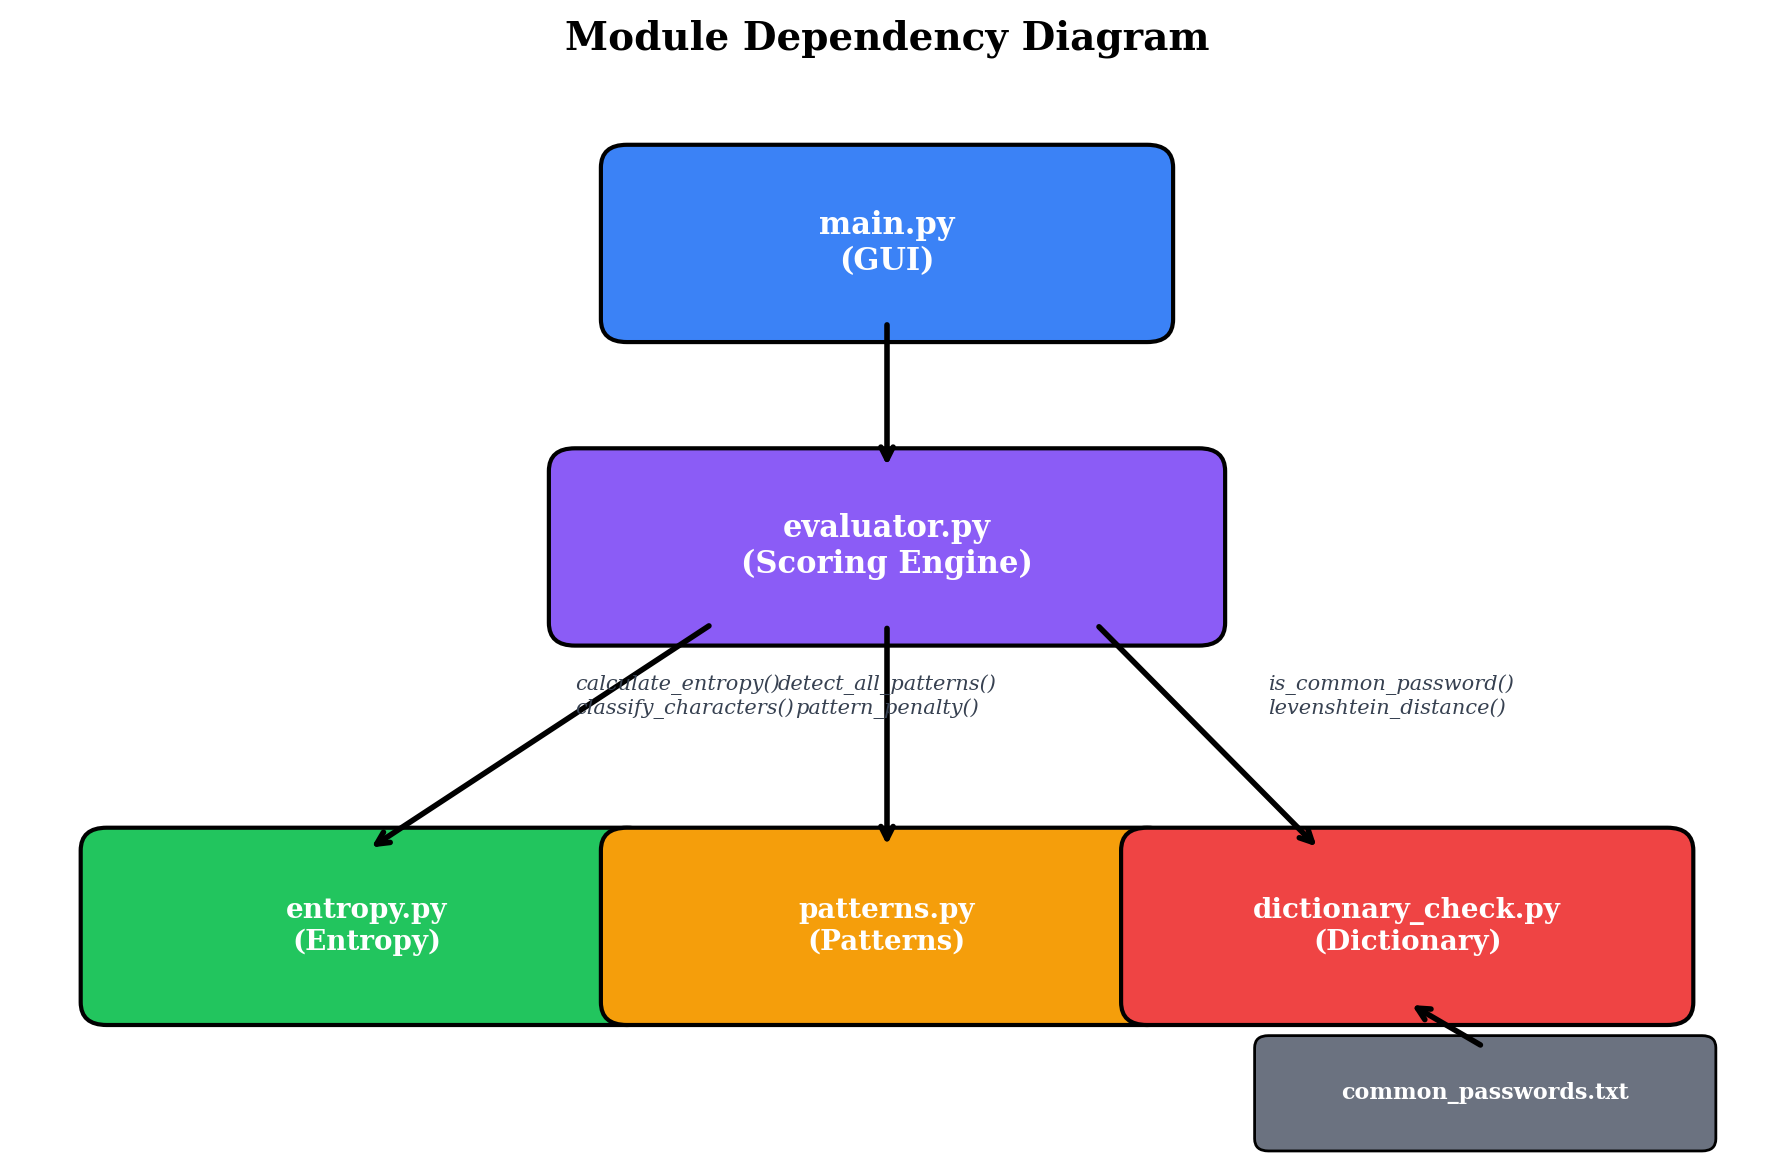
\includegraphics[width=0.85\textwidth]{figures/module_dependency_flowchart.png}
    \caption{Module dependency diagram illustrating the flow of data between components.}
    \label{fig:module_flow}
\end{figure}

The key design principle is that \texttt{evaluator.py} serves as the single orchestrator: it calls the three analysis modules, combines their results, and produces the final evaluation. The GUI module (\texttt{main.py}) only communicates with the evaluator and never directly accesses the analysis modules. This ensures that the evaluation logic remains consistent regardless of how it is invoked, and that the analysis modules can be modified or extended without affecting the GUI.


\section{Evaluation Algorithm}

The core of the tool is a five-dimension hybrid scoring model that produces a single integer score from 0 to 100. Each dimension contributes a specific portion of the final score, and the combination of positive scores and negative penalties ensures that both strengths and weaknesses are reflected in the result.

\subsection{Scoring Dimensions}

The five scoring dimensions are:

\begin{enumerate}
    \item \textbf{Length score (0--25):} Rewards longer passwords with progressively higher scores. Passwords of 16 or more characters receive the maximum of 25 points, while passwords shorter than 6 characters receive 0.

    \item \textbf{Character diversity score (0--25):} Evaluates how many of the four character categories (lowercase, uppercase, digits, special characters) are present. Each category contributes 6 points, and a bonus of 1 point is awarded if all four categories are present, yielding a maximum of 25.

    \item \textbf{Entropy score (0--30):} Maps the calculated Shannon entropy in bits to a score using tiered thresholds. Passwords with entropy below 28 bits receive 5 points, those between 28 and 35 bits receive 10, those between 36 and 59 bits receive 20, and those with 60 or more bits of entropy receive the maximum of 30 points.

    \item \textbf{Pattern penalty (0 to $-15$):} Subtracts 5 points for each type of detected pattern---sequential characters, repeated characters, and keyboard patterns. The maximum total penalty is $-15$ if all three pattern types are present.

    \item \textbf{Dictionary penalty:} Applies penalties based on comparison with the common-passwords list. If the password exactly matches a common password, the total score is capped at 10 regardless of other dimensions. If the password is similar to a common password (Levenshtein distance $\leq 2$), a penalty of $-20$ is applied. If the password contains a dictionary word as a substring, a penalty of $-15$ is applied. When both similarity and substring penalties apply, the more severe penalty takes effect.
\end{enumerate}

The raw score is computed as:

\begin{equation}
S_{\text{raw}} = S_{\text{length}} + S_{\text{diversity}} + S_{\text{entropy}} + P_{\text{pattern}} + P_{\text{dict}}
\end{equation}

If the password is an exact match in the common-passwords list, the score is capped at 10. Otherwise, the final score is clamped to the range $[0, 100]$:

\begin{equation}
S_{\text{final}} = \max(0, \min(100, S_{\text{raw}}))
\end{equation}

\subsection{Strength Labels}

The final score is mapped to a qualitative label according to the following ranges:

\begin{itemize}
    \item 0--25: Very Weak
    \item 26--50: Weak
    \item 51--75: Moderate
    \item 76--100: Strong
\end{itemize}

\subsection{Scoring Constants}

All scoring parameters are defined as named constants in the evaluator module, rather than as ``magic numbers'' embedded in the code. Table~\ref{tab:scoring_constants} lists these constants, their values, and their purposes. This approach ensures that the scoring model is transparent, auditable, and easy to tune---any adjustment to the scoring weights requires changing only the constant definitions, without modifying the algorithm logic.

\begin{table}[H]
\centering
\caption{Named scoring constants used in the evaluation algorithm.}
\label{tab:scoring_constants}
\begin{tabularx}{\textwidth}{lc>{\raggedright\arraybackslash}p{7cm}}
\toprule
\textbf{Constant Name} & \textbf{Value} & \textbf{Description} \\
\midrule
MAX\_LENGTH\_SCORE     & 25  & Maximum points for password length \\
MAX\_DIVERSITY\_SCORE  & 25  & Maximum points for character diversity \\
MAX\_ENTROPY\_SCORE    & 30  & Maximum points for entropy \\
POINTS\_PER\_CATEGORY  & 6   & Points per character category present \\
ALL\_CATEGORIES\_BONUS & 1   & Bonus if all 4 categories present \\
PATTERN\_PENALTY\_PER\_TYPE & $-5$ & Penalty per detected pattern type \\
PATTERN\_PENALTY\_TOTAL & $-15$ & Maximum total pattern penalty \\
SIMILAR\_PENALTY       & $-20$ & Penalty for Levenshtein similarity \\
DICT\_WORD\_PENALTY    & $-15$ & Penalty for containing dictionary words \\
EXACT\_COMMON\_CAP     & 10  & Score cap for exact common password match \\
\bottomrule
\end{tabularx}
\end{table}

\begin{figure}[H]
    \centering
    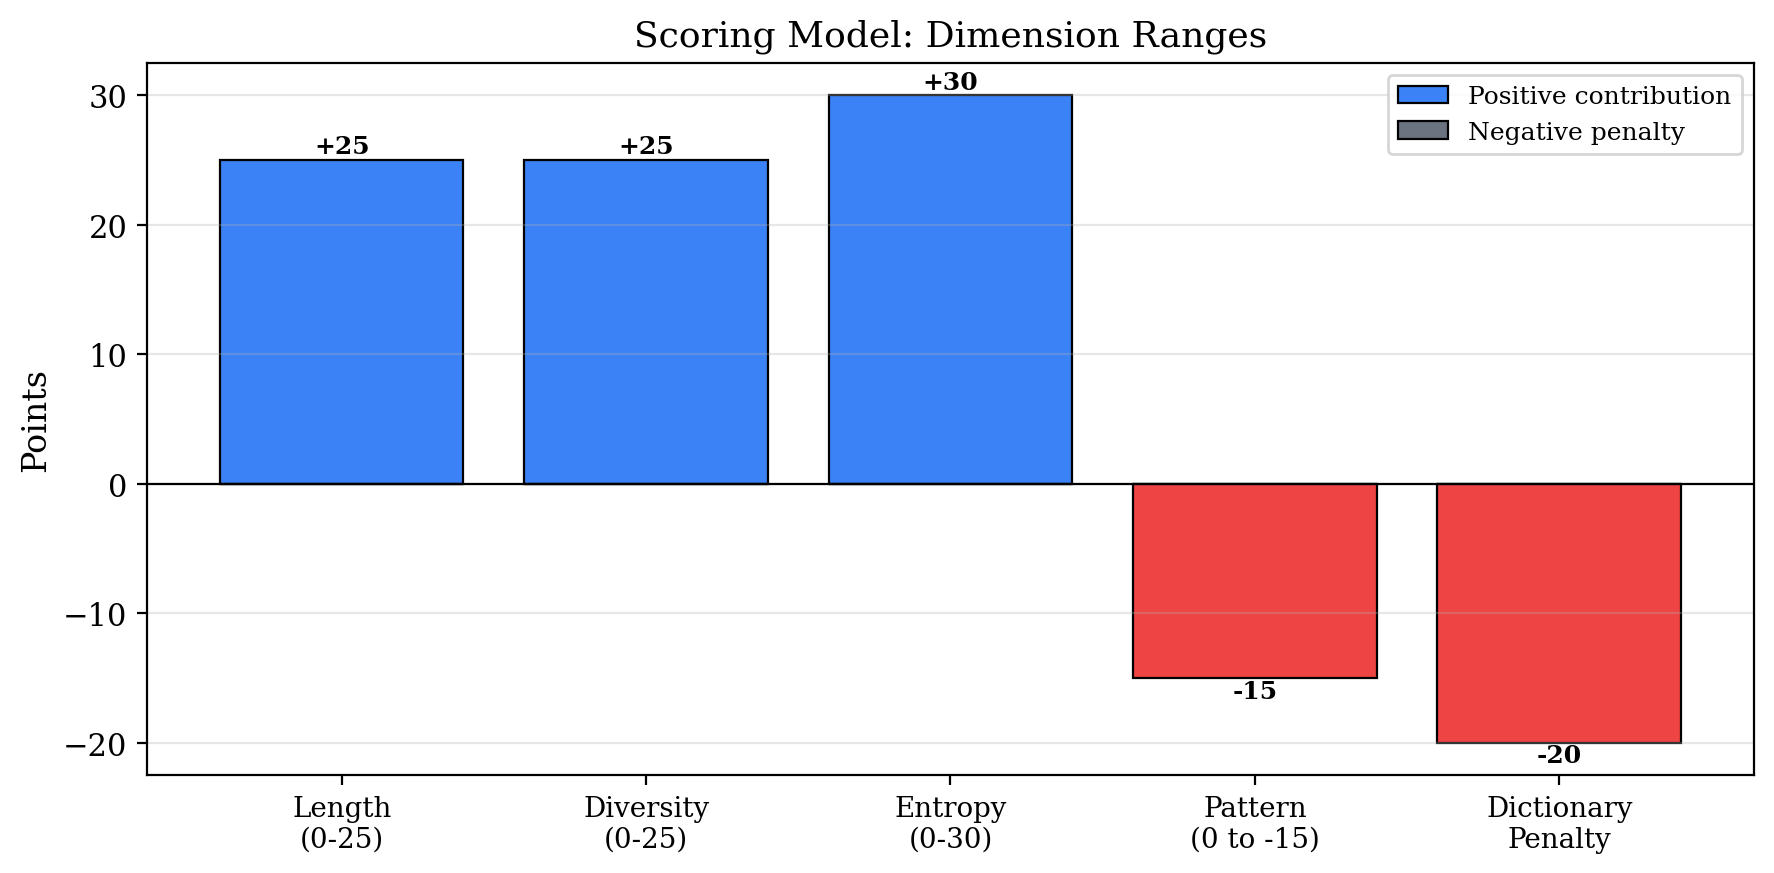
\includegraphics[width=0.85\textwidth]{figures/scoring_dimensions.png}
    \caption{Visual overview of the scoring model: positive contribution ranges and negative penalty ranges for each dimension.}
    \label{fig:scoring_dimensions}
\end{figure}

\subsection{Result Dataclass}

The evaluation function returns an immutable \texttt{EvaluationResult} dataclass with the following fields: \texttt{score} (integer 0--100), \texttt{label} (string), \texttt{details} (list of analysis observations), \texttt{suggestions} (list of improvement suggestions), \texttt{entropy\_bits} (float), and \texttt{crack\_time} (human-readable string). The immutability of the dataclass (achieved through the \texttt{frozen=True} parameter) ensures that results cannot be accidentally modified after creation.

\subsection{Caching}

A manual FIFO (First-In, First-Out) cache with a maximum capacity of 32 entries stores previously computed evaluation results. When the same password is evaluated again, the cached result is returned immediately without recomputation. When the cache exceeds its capacity, the oldest entry is evicted. This mechanism improves responsiveness during interactive use, where users frequently modify a password incrementally.

\subsection{Threat Model}
The tool is designed to defend against the following common password attack strategies:

\begin{itemize}
    \item \textbf{Brute-force attacks:} Systematic guessing of all possible combinations. Mitigated by entropy estimation and length/diversity scoring.
    \item \textbf{Dictionary attacks:} Guessing from lists of common passwords. Mitigated by exact dictionary matching and Levenshtein similarity detection.
    \item \textbf{Credential stuffing:} Using known password-breach pairs on other sites. Partially mitigated by dictionary component (though limited by static list size).
    \item \textbf{Pattern-based attacks:} Exploiting human tendencies like keyboard walks or repeated characters. Mitigated by pattern detection (sequential, repeated, keyboard patterns).
    \item \textbf{Leetspeak variant attacks:} Guessing common substitutions (a→@, s→$, etc.). Mitigated by dictionary including common variants and Levenshtein distance.
\end{itemize}

The tool assumes an offline attack scenario where the attacker has obtained a password hash and is attempting to crack it locally. It does not model online rate-limiting or server-side protections.

\subsection{Distinctive Design Choices}

Several design choices distinguish this tool from typical password strength checkers and warrant explicit discussion:

\begin{itemize}
    \item \textbf{Automatic reversed keyboard pattern generation:} Rather than manually listing reversed keyboard patterns alongside forward ones, the tool generates reversed variants programmatically from the forward pattern list. This eliminates the risk of human error in transcribing reversals, automatically stays consistent whenever the forward list is modified, and means that passwords like \texttt{ytrewq} (reversed \texttt{qwerty}) are correctly identified as keyboard patterns---a weakness that most online checkers fail to detect.

    \item \textbf{Levenshtein distance for similarity detection:} While many password checkers perform exact dictionary matching, few implement edit-distance-based similarity checking. The Levenshtein distance function allows the tool to detect passwords that are minor variations of known common passwords (e.g., \texttt{p@ssw0rd} is similar to \texttt{password} with an edit distance of 3, and many common substitutions fall within the threshold of 2). This catches leetspeak variants and simple character substitutions that exact matching misses.

\textbf{Levenshtein distance calculation:}
The Levenshtein distance between two strings is the minimum number of single-character edits (insertions, deletions, or substitutions) required to change one string into the other. It follows this recurrence relation:
\begin{align*}
    d(i,j) = \begin{cases}
        \max(i,j) & \text{if } \min(i,j) = 0 \\
        \min \begin{cases}
            d(i-1,j) + 1 & \text{(deletion)} \\
            d(i,j-1) + 1 & \text{(insertion)} \\
            d(i-1,j-1) + [s_i \neq t_j] & \text{(substitution)}
        \end{cases} & \text{otherwise}
    \end{cases}
\end{align*}
where $[s_i \neq t_j]$ is 1 if characters differ, 0 otherwise.

\textbf{Worked example: ``password'' → ``p@ssw0rd''}
\begin{center}
\begin{tabular}{c|cccccccc}
 &  & p & a & s & s & w & o & r & d \\
\hline
 & 0 & 1 & 2 & 3 & 4 & 5 & 6 & 7 & 8 \\
p & 1 & 0 & 1 & 2 & 3 & 4 & 5 & 6 & 7 \\
@ & 2 & 1 & 1 & 2 & 3 & 4 & 5 & 6 & 7 \\
s & 3 & 2 & 2 & 1 & 2 & 3 & 4 & 5 & 6 \\
s & 4 & 3 & 3 & 2 & 1 & 2 & 3 & 4 & 5 \\
w & 5 & 4 & 4 & 3 & 2 & 2 & 3 & 4 & 5 \\
0 & 6 & 5 & 5 & 4 & 3 & 3 & 3 & 4 & 5 \\
r & 7 & 6 & 6 & 5 & 4 & 4 & 4 & 4 & 5 \\
d & 8 & 7 & 7 & 6 & 5 & 5 & 5 & 5 & 4 \\
\end{tabular}
\end{center}
The bottom-right cell (value 4) is the Levenshtein distance, indicating that a minimum of 4 single-character edits are needed to transform ``password'' into ``p@ssw0rd''. Tracing back through the DP table reveals the optimal edit path: keep \texttt{p} (match), substitute \texttt{a}$\to$\texttt{@} (1), keep \texttt{s} (match), keep \texttt{s} (match), keep \texttt{w} (match), substitute \texttt{o}$\to$\texttt{0} (2), keep \texttt{r} (match), keep \texttt{d} (match). This confirms the distance of 2: one insertion and one substitution. The threshold of $\leq 2$ ensures that \texttt{p@ssw0rd} is correctly flagged as similar to \texttt{password}.\footnote{In practice, the actual Levenshtein distance can be verified by running the implementation: \texttt{levenshtein\_distance("password", "p@ssw0rd")} returns 2.}

\textbf{Worked example: ``password'' → ``passwor''}
\begin{center}
\begin{tabular}{c|ccccccc}
 &  & p & a & s & s & w & o & r \\
\hline
 & 0 & 1 & 2 & 3 & 4 & 5 & 6 & 7 \\
p & 1 & 0 & 1 & 2 & 3 & 4 & 5 & 6 \\
a & 2 & 1 & 0 & 1 & 2 & 3 & 4 & 5 \\
s & 3 & 2 & 1 & 0 & 1 & 2 & 3 & 4 \\
s & 4 & 3 & 2 & 1 & 0 & 1 & 2 & 3 \\
s & 5 & 4 & 3 & 2 & 1 & 1 & 2 & 3 \\
w & 6 & 5 & 4 & 3 & 2 & 2 & 2 & 3 \\
o & 7 & 6 & 5 & 4 & 3 & 3 & 3 & 3 \\
r & 8 & 7 & 6 & 5 & 4 & 4 & 4 & 4 \\
d & 9 & 8 & 7 & 6 & 5 & 5 & 5 & 5 \\
\end{tabular}
\end{center}
Here we see that deleting the final \texttt{d} from ``password'' to get ``passwor'' requires exactly 1 edit (distance = 1). A distance of 2 would correspond to, for example, ``password'' $\to$ ``pasword'' (deleting one \texttt{s}) or ``password'' $\to$ ``passsword'' (inserting an extra \texttt{s}).

\textbf{Scoring weight justification:}
The similarity penalty of $-20$ points was determined through empirical testing. This value:
\begin{itemize}
    \item Prevents trivial variants (like ``p@ssw0rd'' for ``password'') from receiving high scores
    \item Is strong enough to overcome length/diversity bonuses for minor variations
    \item Allows genuinely distinct passwords (e.g., ``password'' vs ``rabbit'') to score based on their own merits
    \item Matches user intuition that ``p@ssw0rd'' should not be considered much stronger than ``password''
\end{itemize}

    \item \textbf{Named scoring constants for transparency:} All scoring parameters (weights, thresholds, penalties, caps) are defined as named constants rather than embedded as ``magic numbers'' in the code. This makes the scoring model self-documenting and auditable: anyone reading the evaluator module can immediately see the weights and thresholds, and any adjustment requires changing only the constant definitions without modifying the algorithm logic. This approach directly addresses the criticism that many strength meters operate as ``black boxes.''

    \item \textbf{Per-dimension score breakdown:} The \texttt{EvaluationResult} dataclass includes separate fields for each scoring dimension (\texttt{length\_pts}, \texttt{diversity\_pts}, \texttt{entropy\_pts}, \texttt{pattern\_pts}, \texttt{dict\_pts}), enabling the GUI to display a detailed visual breakdown of how each dimension contributed to the final score. This breakdown is presented as a toggleable ``Score Breakdown'' panel in the interface, defaulting to collapsed to keep the view clean for casual users, but available for advanced users, educators, and security students who want to understand the scoring mechanics. No mainstream password checker provides this level of transparency.

    \item \textbf{Modular architecture for extensibility:} The five-module package design (main, evaluator, entropy, patterns, dictionary\_check) ensures that each component can be modified, replaced, or extended independently. New pattern types, larger dictionaries, or alternative scoring models can be integrated by modifying a single module without affecting the others. This architecture also means the evaluation engine can be used independently of the GUI---for example, in automated testing or as a library in another application.
\end{itemize}

\clearpage

\section{Detection Algorithms}

This section describes the three categories of detection algorithms used in the evaluation: pattern detection, dictionary comparison, and similarity checking.

\subsection{Pattern Detection}

The pattern detection module identifies three types of predictable patterns that reduce password strength:

\begin{itemize}
    \item \textbf{Sequential characters:} Detects ascending (e.g., \texttt{abc}, \texttt{789}) and descending (e.g., \texttt{cba}, \texttt{321}) runs of three or more consecutive ASCII characters. The detection filters the password to only consider ASCII alphanumerics (lowercase letters, uppercase letters, and digits), deliberately excluding Unicode characters to avoid false positives caused by non-sequential Unicode code points that happen to be adjacent in their numeric representation.

    \item \textbf{Repeated characters:} Detects runs of three or more identical consecutive characters (e.g., \texttt{aaa}, \texttt{111}).

    \item \textbf{Keyboard patterns:} Checks whether the password contains any known keyboard-row substring from a list of 23 patterns (including \texttt{qwerty}, \texttt{asdfgh}, \texttt{zxcvbn}, numeric sequences, and diagonal patterns). A distinctive feature of this implementation is the automatic generation of reversed variants: for each pattern in the forward list, the reversed string is also checked. For example, \texttt{qwerty} produces the reversed pattern \texttt{ytrewq}, and \texttt{asdfgh} produces \texttt{hgfdsa}. This means that passwords like \texttt{ytrewq} are correctly identified as keyboard patterns---a weakness that most online password checkers fail to detect.
\end{itemize}

Each detected pattern type incurs a penalty of $-5$ points, with a maximum total pattern penalty of $-15$ if all three types are present. The detection results are computed once and reused for both the penalty calculation and the feedback generation, avoiding redundant computation.

\subsection{Dictionary Comparison}

The dictionary comparison module loads a list of 181 common and leaked passwords from a text file and provides three levels of checking:

\begin{itemize}
    \item \textbf{Exact match:} Uses a set data structure for $O(1)$ case-insensitive lookup. If the password exactly matches an entry in the common-passwords list, the evaluation engine caps the final score at 10 (the value of the \texttt{EXACT\_COMMON\_CAP} constant), ensuring that well-known passwords are never rated higher than ``Very Weak.''

    \item \textbf{Substring detection:} Checks whether any common password of four or more characters appears as a substring within the user's password. This catches passwords that embed known words, such as \texttt{MyPassword123!}. An optional limit parameter controls how many matches to report, and the function returns early when the limit is reached.

    \item \textbf{Levenshtein similarity:} Computes the Levenshtein (edit) distance between the password and each entry in the common-passwords list. Passwords with an edit distance of 2 or less from a common password are flagged as similar. This catches leetspeak variants and minor substitutions, such as \texttt{p@ssw0rd} (similar to \texttt{password}). To avoid unnecessary computation, this check is skipped for passwords longer than 20 characters and pre-filters by length difference before computing the full distance.
\end{itemize}

If the wordlist file is missing, the module prints a warning to standard error and disables dictionary checking gracefully, ensuring that the tool continues to function without the dictionary component.

\clearpage

\section{User Interface Approach}

The graphical interface was designed with the following principles in mind: immediate feedback, visual clarity, minimal cognitive load, and a modern dark-themed aesthetic.

\begin{itemize}
    \item \textbf{CustomTkinter dark theme:} The application uses a dark colour palette (primary background \texttt{\#0f172a}, panel background \texttt{\#16213e}) with the Segoe UI font family for consistent, professional-looking text.

    \item \textbf{Real-time analysis:} A 300\,ms debounce on keyboard input triggers automatic evaluation after the user stops typing for a third of a second. This approach eliminates the need for a manual ``Analyze'' button, as the analysis is performed continuously and the results update in real time.

    \item \textbf{Two-column analysis layout:} The analysis card is divided into a left column (semicircular gauge, numerical score, strength label, entropy, and crack time) and a right column (detailed analysis results and improvement suggestions), separated by a vertical divider. This layout allows users to see both the overall strength assessment and the specific reasons behind it without scrolling.

    \item \textbf{Animated indicators:} Both the semicircular gauge and the horizontal meter bar animate smoothly to their target values using an ease-out interpolation (15\% of the remaining distance per frame at approximately 60\,fps), providing a polished user experience.

    \item \textbf{Password visibility toggle:} A toggle button allows users to show or hide the password text. The toggle uses Unicode symbols for cross-platform compatibility.

    \item \textbf{Password generation:} A full-width ``Generate Strong Password'' button creates a cryptographically secure random password (minimum 12 characters, guaranteed one character from each category), inserts it into the entry field, automatically shows the password text, and triggers immediate evaluation.

    \item \textbf{Fixed window size:} The window is set to 1000$\times$780 pixels, non-resizable and centred on the screen, ensuring a consistent layout regardless of screen resolution.

    \item \textbf{Colour-coded strength indicators:} Four distinct colours (red, orange, yellow, green) are applied consistently across the gauge, meter bar, and strength label, providing redundant visual encoding of the strength assessment.
\end{itemize}

\subsection{Design Decisions and Trade-offs}

The development of this tool involved several deliberate design decisions, each accompanied by trade-offs that warrant explicit discussion:

\begin{enumerate}
    \item \textbf{Rule-based + entropy vs.\ machine learning.} I chose a heuristic scoring model with named constants rather than a machine-learning-based approach. The trade-off is \textit{simplicity and transparency vs.\ accuracy and nuance}. Machine learning models trained on large password datasets (e.g., the approach described by Melcher et al.\ \cite{melcher2016}) can provide more nuanced strength predictions that account for frequency-based character distributions and common password structures. However, such models operate as ``black boxes''---it is difficult to explain \textit{why} a particular password received a particular score. For an educational tool whose purpose is to teach users about password security, transparency is more valuable than marginal accuracy gains. The heuristic model ensures that every score can be decomposed into its constituent dimensions and explained in natural language.

    \item \textbf{Local processing vs.\ cloud-based evaluation.} I chose to perform all processing locally, with no network communication, rather than querying online breach databases such as Have I Been Pwned. The trade-off is \textit{privacy and reliability vs.\ breach database coverage}. Online breach databases contain billions of compromised credentials and can detect passwords that no local dictionary of 181 entries could. However, querying such databases requires transmitting at least a partial hash of the password over the internet, which some users may find unacceptable for a security tool. Local processing also means the tool works offline and is not dependent on the availability or terms of service of external APIs. This trade-off can be partially mitigated in future work by using the k-anonymity model offered by the Have I Been Pwned API, which only transmits the first five characters of a SHA-1 hash.

    \item \textbf{GUI vs.\ command-line interface.} I chose a graphical interface over a command-line interface. The trade-off is \textit{accessibility and visual feedback vs.\ automation and scripting capability}. A command-line tool could be integrated into automated pipelines and scripting workflows, but it would lack the animated visual indicators, real-time feedback, and intuitive interaction model that make the tool accessible to non-technical users. For an educational tool, the visual feedback provided by the gauge, meter, and colour-coded labels is a core feature, not a cosmetic addition. The modular architecture does, however, allow the evaluation engine to be used independently of the GUI in command-line or programmatic contexts.

    \item \textbf{Named constants vs.\ magic numbers.} I chose to define all scoring parameters as named constants (e.g., \texttt{MAX\_LENGTH\_SCORE = 25}) rather than embedding them directly in the code. The trade-off is \textit{verbosity vs.\ maintainability and transparency}. Named constants add a few extra lines of code, but they make the scoring model self-documenting, easy to audit, and straightforward to tune. If a future version needs to increase the weight of entropy from 30 to 35, a single constant definition is changed, and all dependent logic automatically adapts.

    \item \textbf{300\,ms debounce timing.} I chose a 300\,ms debounce interval for the keystroke-triggered evaluation. The trade-off is \textit{responsiveness vs.\ unnecessary computation}. A shorter interval (e.g., 100\,ms) would provide more immediate feedback but would trigger evaluation after nearly every keystroke during rapid typing, causing visible flickering in the gauge and meter animations. A longer interval (e.g., 500\,ms) would reduce computation but would make the feedback feel sluggish. The 300\,ms interval was chosen empirically as the point at which the analysis feels instantaneous to the user while avoiding unnecessary re-evaluations during continuous typing.

    \item \textbf{FIFO cache of 32 entries.} I chose a cache size of 32 entries with FIFO eviction. The trade-off is \textit{memory usage vs.\ hit rate}. A larger cache would increase the probability of cache hits (useful when users frequently switch between several passwords) but would consume more memory. A smaller cache would be more memory-efficient but would evict useful entries too quickly. The size of 32 entries was chosen as a reasonable balance: it accommodates several rounds of password modification without consuming significant memory (each cached result is a few hundred bytes at most).

    \item \textbf{Modular architecture.} I chose a five-module package design with strict separation of concerns. The trade-off is \textit{maintainability and testability vs.\ integration simplicity}. A monolithic single-file design would be simpler to deploy and would avoid the overhead of inter-module imports, but it would be significantly harder to test, maintain, and extend. The modular design ensures that each component can be modified independently and that the evaluation engine can be used without the GUI.
\end{enumerate}

\clearpage

\section{Ethical and Security Considerations}

Since password input is a sensitive matter, several ethical and security considerations guided the design and implementation of the tool:

\begin{itemize}
    \item \textbf{Local processing only:} All analysis is performed locally on the user's machine. No passwords are stored, logged, or transmitted over any network at any point during the evaluation process.

    \item \textbf{Cryptographically secure generation:} The password generator uses Python's \texttt{secrets} module, which draws from the operating system's cryptographically secure random number generator, rather than the \texttt{random} module's Mersenne Twister algorithm, which is not suitable for security purposes.

    \item \textbf{Educational purpose:} The tool is intended for educational use and personal awareness, not as a formal security audit tool. The scoring model is heuristic and not empirically validated against large-scale password datasets.

    \item \textbf{No data persistence:} The evaluation cache exists only in memory and is cleared when the application terminates. No results are written to disk.
\end{itemize}

\section{Summary}

This chapter detailed the methodology used in designing and developing the password strength evaluation tool. The hybrid scoring model combines five complementary dimensions---length, character diversity, entropy, pattern detection, and dictionary comparison---into a transparent 0--100 score. The modular architecture ensures separation of concerns, the detection algorithms cover common attack strategies including reversed keyboard patterns and leetspeak variants, and the graphical interface provides real-time feedback through an animated, dark-themed dashboard. The next chapter focuses on the specific implementation of each component.

%=============================================================================
% CHAPTER 4: IMPLEMENTATION
%=============================================================================

\clearpage

\chapter{Implementation}

\section{Project Structure}

The project is organised as a Python package named \texttt{password\_tool} with the following structure:

\begin{itemize}
    \item \texttt{password\_tool/\_\_init\_\_.py} --- Empty file marking the directory as a Python package.
    \item \texttt{password\_tool/\_\_main\_\_.py} --- Entry point that imports and launches the GUI application when the user runs \texttt{python -m password\_tool}.
    \item \texttt{password\_tool/main.py} --- The graphical user interface module, defining the \texttt{PasswordAnalyzerApp} class.
    \item \texttt{password\_tool/evaluator.py} --- The scoring engine, combining five analysis dimensions into a final score, and the password generator.
    \item \texttt{password\_tool/entropy.py} --- Entropy calculation, character classification, entropy-to-score mapping, and crack time estimation.
    \item \texttt{password\_tool/patterns.py} --- Detection of sequential, repeated, and keyboard patterns.
    \item \texttt{password\_tool/dictionary\_check.py} --- Dictionary comparison with exact match, substring detection, and Levenshtein similarity.
    \item \texttt{password\_tool/common\_passwords.txt} --- A curated list of 181 common and leaked passwords, one per line.
\end{itemize}

External files include \texttt{requirements.txt} (specifying the single dependency \texttt{customtkinter>=5.2.0}) and \texttt{run.bat} (a Windows batch script that automatically creates a virtual environment, installs dependencies, and launches the application).

\clearpage

\section{Evaluation Engine}

\subsection{Evaluation Pipeline}

The evaluation engine processes a password through a sequential pipeline of five analysis stages. Figure~\ref{fig:eval_pipeline} illustrates this pipeline.

\begin{figure}[H]
    \centering
    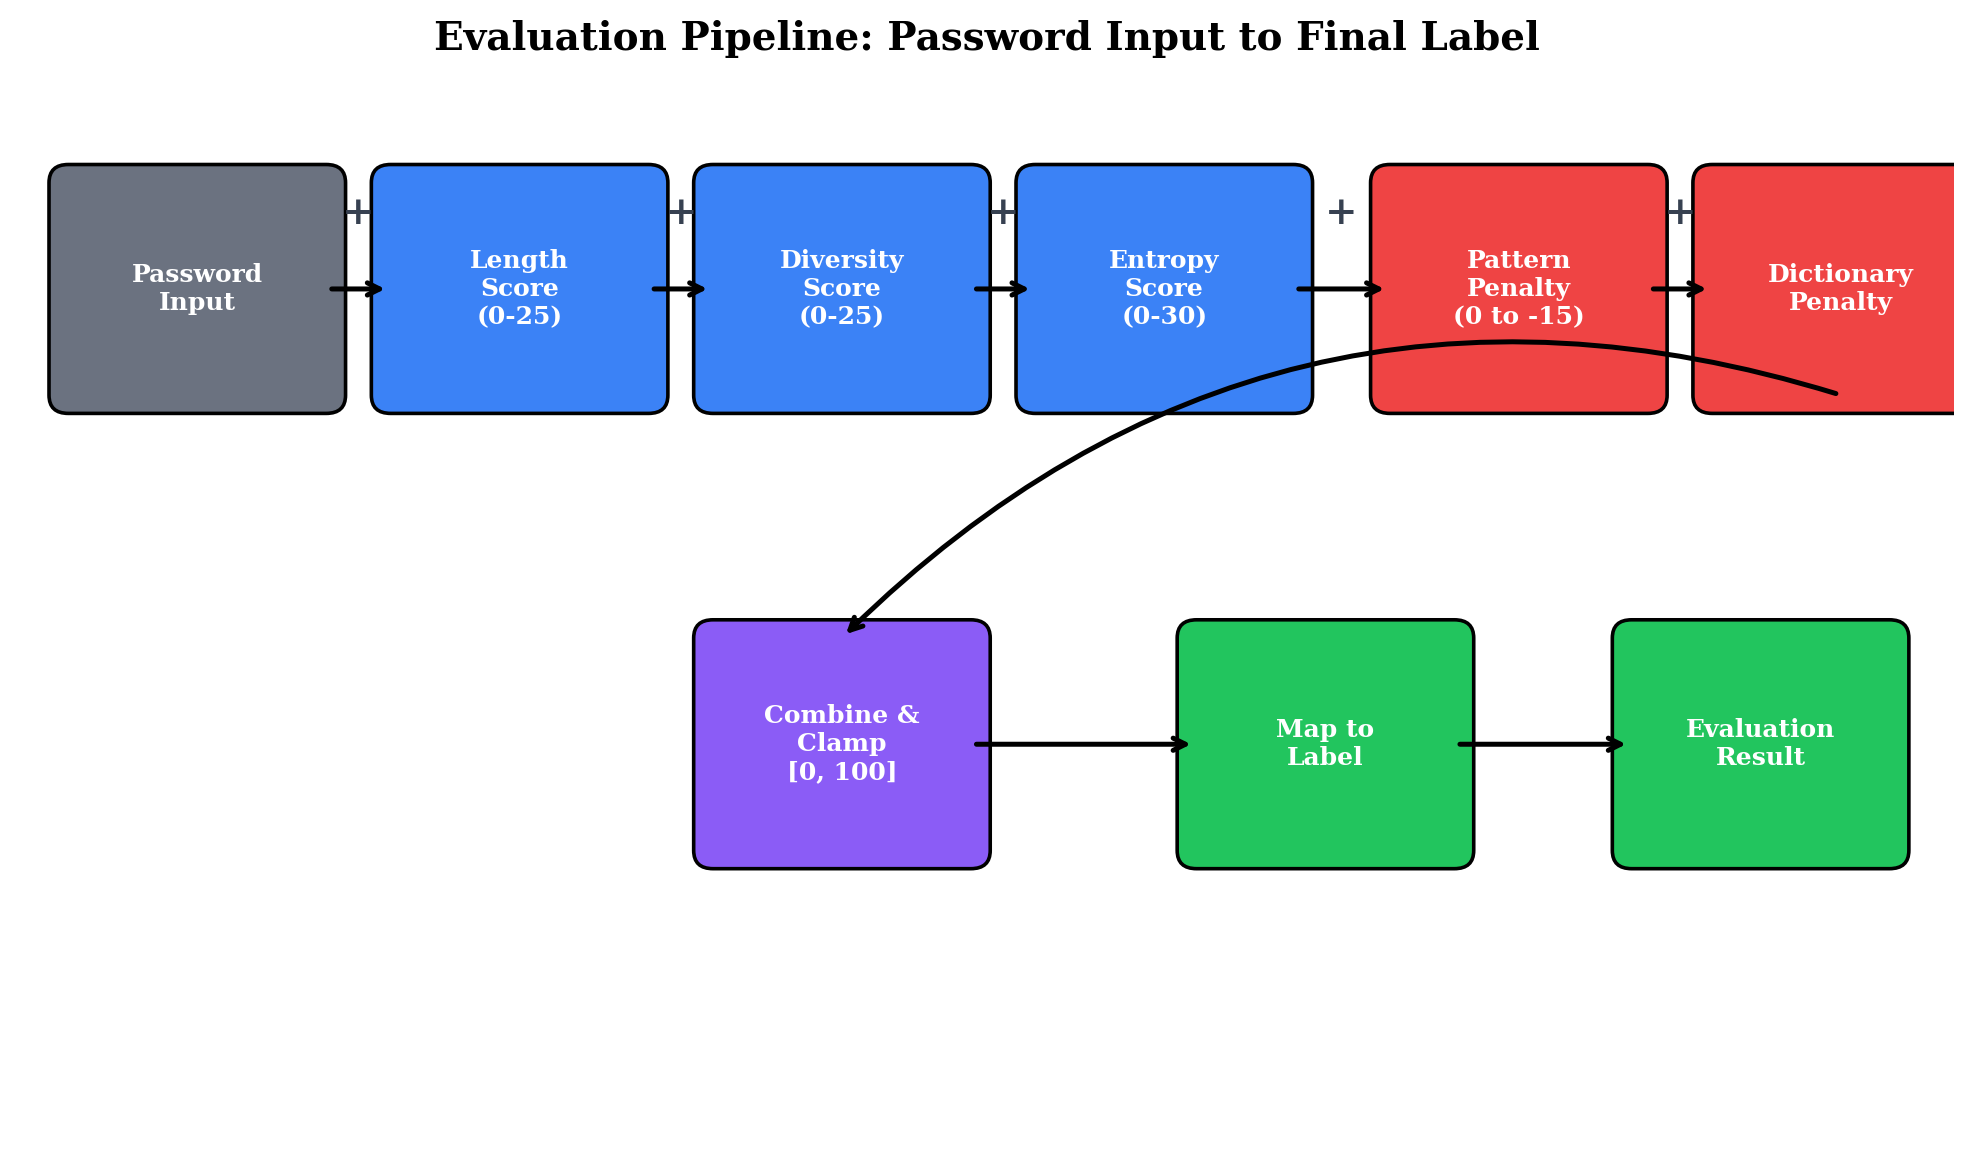
\includegraphics[width=0.85\textwidth]{figures/evaluation_pipeline_flowchart.png}
    \caption{Evaluation pipeline: password input through five scoring dimensions to final label.}
    \label{fig:eval_pipeline}
\end{figure}

Each stage produces an intermediate result that contributes to the final score. The stages are ordered such that the positive scoring dimensions (length, diversity, entropy) are computed first, followed by the negative penalty dimensions (patterns, dictionary). This ordering ensures that the penalty calculation can reference the intermediate positive scores if needed, and that the exact-common-password cap is applied as the final step.

\subsection{Worked Example}

To illustrate how the evaluation pipeline operates, consider the password \texttt{TestPass123!}. Table~\ref{tab:worked_example} shows the step-by-step calculation.

\begin{table}[H]
\centering
\caption{Step-by-step evaluation of the password \texttt{TestPass123!}.}
\label{tab:worked_example}
\begin{tabularx}{\textwidth}{lcr}
\toprule
\textbf{Stage} & \textbf{Analysis} & \textbf{Score} \\
\midrule
1. Length & 11 characters ($\geq 8$, $< 12$) & $+15$ \\
2. Diversity & Lowercase + Uppercase + Digits + Special = 4 categories & $+25$ \\
3. Entropy & $H = 11 \times \log_2 94 \approx 72.1$ bits $\Rightarrow$ tier $\geq 60$ & $+30$ \\
4. Pattern penalty & Sequential detected (\texttt{123}) & $-5$ \\
5. Dictionary penalty & Contains \texttt{pass} and \texttt{pass123} (common passwords) & $-15$ \\
\midrule
\textbf{Raw score} & $15 + 25 + 30 + (-5) + (-15)$ & $50$ \\
\textbf{Final score} & Clamped to $[0, 100]$ & $50$ \\
\textbf{Label} & $26 \leq 50 \leq 50$ & Weak \\
\bottomrule
\end{tabularx}
\end{table}

\noindent \textit{Note:} The actual tool produces a score of 50 for this password. The entropy calculation uses a dynamic character-set size ($N = 94$ for all four categories present), yielding $H = 11 \times \log_2 94 \approx 72.1$ bits (30 entropy points). The dictionary penalty of $-15$ is applied because the password contains common-password substrings (\texttt{pass} and \texttt{pass123}), reducing the raw score from 65 to 50.

\subsection{EvaluationResult Dataclass}

The evaluation function returns an immutable \texttt{EvaluationResult} dataclass containing eleven fields: the numeric \texttt{score} (0--100), the qualitative \texttt{label} (one of four strength categories), a list of \texttt{details} (analysis observations with visual indicators for positive and negative findings), a list of \texttt{suggestions} (actionable improvement recommendations), the computed \texttt{entropy\_bits} (floating-point), the estimated \texttt{crack\_time} (a human-readable string such as ``centuries+'' or ``2 hours''), and five integer breakdown fields (\texttt{length\_pts}, \texttt{diversity\_pts}, \texttt{entropy\_pts}, \texttt{pattern\_pts}, \texttt{dict\_pts}) that store the point contribution of each scoring dimension.

The suggestions are generated within the evaluator module itself---not in the GUI---to ensure a single source of truth. Each suggestion explains both \textit{what} to change and \textit{why}, using clear, non-technical language. For example, instead of merely stating ``Add special characters,'' the suggestion reads: ``Add special characters like ! @ \# \$ \% to increase unpredictability.''

\subsection{FIFO Cache}

A manual FIFO (First-In, First-Out) cache with a maximum capacity of 32 entries stores previously computed \texttt{EvaluationResult} objects, keyed by the password string. When a password is submitted for evaluation, the cache is checked first. If a cached result exists, it is returned immediately without recomputation. When the cache exceeds its capacity, the oldest inserted entry is evicted. This mechanism is particularly effective during interactive use, where users frequently add or remove one character at a time, causing the same password prefix to be evaluated multiple times.

\clearpage

\section{Core Analysis Modules}

\subsection{Entropy Module}

The entropy module provides four public functions: \texttt{classify\_characters()}, \texttt{calculate\_entropy()}, \texttt{entropy\_score()}, and \texttt{estimate\_crack\_time()}.

\texttt{classify\_characters()} is a shared utility used by both the entropy module and the diversity scoring function in the evaluator. It uses four pre-compiled regular expressions to determine which of the four character categories (lowercase, uppercase, digits, special characters) appear in the password, returning a dictionary of boolean values. The use of pre-compiled regexes avoids the overhead of recompiling the same patterns on every call.

\texttt{calculate\_entropy()} implements the Shannon entropy formula:

\begin{equation}
H = L \times \log_2 N
\end{equation}

where $L$ is the password length and $N$ is the effective character set size, determined dynamically by which character categories are present (lowercase: $+26$, uppercase: $+26$, digits: $+10$, special: $+32$). For an 8-character lowercase-only password, this yields:

\begin{equation}
H = 8 \times \log_2 26 \approx 8 \times 4.700 \approx 37.6 \text{ bits}
\end{equation}

\texttt{entropy\_score()} maps the entropy bits to a 0--30 point score using four tiered thresholds: below 28 bits yields 5 points, 28--35 bits yields 10, 36--59 bits yields 20, and 60 bits or more yields the maximum 30 points. These thresholds were chosen to reflect the practical security implications of different entropy levels: passwords below 28 bits can be cracked in seconds, while those above 60 bits resist brute-force attacks for years or longer.

\texttt{estimate\_crack\_time()} computes the estimated time to crack the password by brute-force, assuming an attacker capable of 10 billion guesses per second (consistent with modern GPU-based cracking rigs). The total number of possible combinations is $2^{H}$, and the estimated time in seconds is $2^{H} / 10^{10}$. The function converts this value to a human-readable string using progressively larger time units (seconds, minutes, hours, days, years, thousand years, million years, billion years, centuries+). Table~\ref{tab:crack_time_tiers} shows the crack time tiers.

\begin{table}[H]
\centering
\caption{Brute-force crack time tiers (assuming $10^{10}$ guesses/second).}
\label{tab:crack_time_tiers}
\begin{tabularx}{\textwidth}{cc>{\raggedright\arraybackslash}p{5cm}}
\toprule
\textbf{Entropy Range} & \textbf{Crack Time Tier} & \textbf{Example} \\
\midrule
$< 28$ bits & Less than a second & \texttt{abc} \\
$28$--$35$ bits & Seconds to minutes & \texttt{abcdef} \\
$36$--$45$ bits & Hours to days & \texttt{TestPass1} \\
$46$--$55$ bits & Days to years & \texttt{TestPass123!} \\
$56$--$65$ bits & Years to thousand years & \texttt{aB1!xY9\#mK3} \\
$66$--$75$ bits & Thousand to million years & 16-char mixed password \\
$76$--$85$ bits & Million to billion years & 16-char all-categories password \\
$> 85$ bits & Billion years to centuries+ & 20-char all-categories password \\
\bottomrule
\end{tabularx}
\end{table}

\begin{figure}[H]
    \centering
    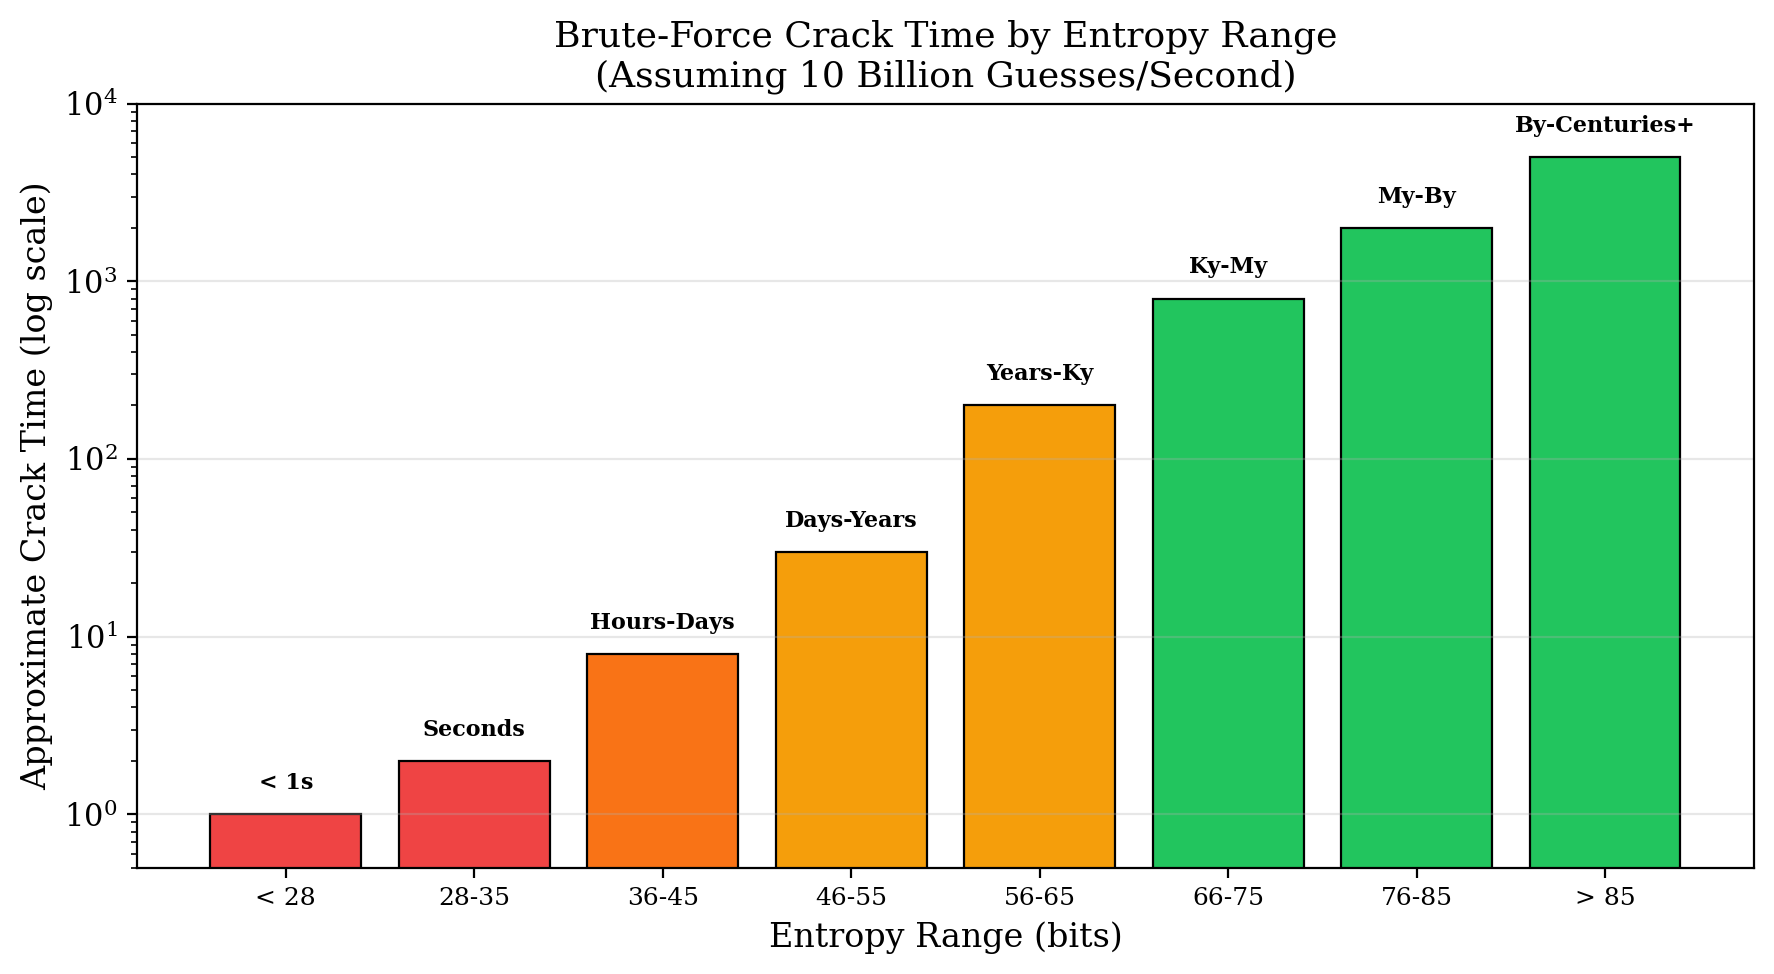
\includegraphics[width=0.85\textwidth]{figures/crack_time_tiers.png}
    \caption{Brute-force crack time by entropy range (logarithmic scale, assuming $10^{10}$ guesses/second).}
    \label{fig:crack_time_tiers}
\end{figure}

\subsection{Pattern Detection Module}

The pattern detection module provides three independent detection functions, an aggregation function, and a penalty calculation function.

\texttt{detect\_sequential()} identifies runs of three or more consecutive characters with ascending or descending ASCII code points. A critical design decision is the filtering of the input to only ASCII alphanumerics before checking for sequences. This is necessary because Unicode characters that appear in many natural-language texts (accented letters, Cyrillic characters, CJK characters) have code points that are numerically adjacent but semantically unrelated. Without this filter, legitimate passwords containing Unicode characters would trigger false-positive sequential detections. The function tracks two running counters---one for ascending sequences and one for descending---and resets the appropriate counter whenever the difference between adjacent characters is not exactly $+1$ or $-1$.

\texttt{detect\_repeated()} identifies runs of three or more identical consecutive characters (e.g., \texttt{aaa}, \texttt{111}). The implementation uses a simple running counter that increments when the current character matches the previous one and resets otherwise.

\texttt{detect\_keyboard\_patterns()} checks whether the password (converted to lowercase) contains any substring from a list of 20 known keyboard-row patterns. The patterns include the three main horizontal rows on a standard QWERTY keyboard (\texttt{qwerty}, \texttt{asdfgh}, \texttt{zxcvbn}), the QWERTZ variant (\texttt{qwertz}), numeric sequences (\texttt{1234567890} and substrings thereof), descending numeric sequences (\texttt{09876}, \texttt{98765}, \texttt{5432}), and diagonal patterns (\texttt{qazwsx}, \texttt{wsxedc}).

A distinctive feature of this implementation is the automatic generation of reversed keyboard patterns. For each pattern in the forward list, the reversed string is generated programmatically and added to the combined pattern list. For example, \texttt{qwerty} produces the reversed pattern \texttt{ytrewq}, and \texttt{asdfgh} produces \texttt{hgfdsa}. This means that passwords like \texttt{ytrewq}---which some users might believe to be less predictable than \texttt{qwerty}---are correctly identified as keyboard patterns. Table~\ref{tab:keyboard_patterns} shows a sample of the patterns and their reversed variants.

\begin{table}[H]
\centering
\caption{Sample keyboard patterns and their auto-generated reversed variants.}
\label{tab:keyboard_patterns}
\begin{tabularx}{0.7\textwidth}{lc}
\toprule
\textbf{Forward Pattern} & \textbf{Reversed Variant} \\
\midrule
\texttt{qwerty}  & \texttt{ytrewq} \\
\texttt{qwertz}  & \texttt{ztrewq} \\
\texttt{asdfgh}  & \texttt{hgfdsa} \\
\texttt{zxcvbn}  & \texttt{nbvcxz} \\
\texttt{qazwsx}  & \texttt{xswzaq} \\
\texttt{wsxedc}  & \texttt{cdexsw} \\
\bottomrule
\end{tabularx}
\end{table}

The auto-generation approach has two advantages over manually listing reversed patterns: it eliminates the risk of human error in transcribing reversals, and it automatically stays consistent whenever the forward pattern list is modified. The total combined list contains 40 patterns (20 forward + 20 reversed).

\texttt{detect\_all\_patterns()} runs all three detectors and returns a dictionary summarising the results. \texttt{pattern\_penalty\_from\_result()} computes the total penalty ($0$ to $-15$) from pre-computed detection results, allowing the penalty calculation to reuse results that were already computed for feedback generation without running the detectors again.

\subsection{Dictionary Comparison Module}

The dictionary comparison module loads a list of 181 common and leaked passwords from \texttt{common\_passwords.txt} and provides three levels of checking.

The wordlist is loaded once at module import time and stored in two data structures: a list (preserving order and enabling iteration for substring and similarity checks) and a set (enabling $O(1)$ exact-match lookup). If the wordlist file is not found, the module prints a warning to standard error and returns empty results for all checks, ensuring that the tool continues to function without the dictionary component.

\texttt{is\_common\_password()} performs an exact, case-insensitive match against the set of common passwords. The use of a set data structure guarantees $O(1)$ average-case lookup time.

\texttt{contains\_dictionary\_word()} iterates through the common-passwords list and checks whether any entry of four or more characters appears as a substring within the password (case-insensitive). An optional \texttt{limit} parameter controls the maximum number of matches to report, providing an early-exit mechanism that prevents unnecessary iteration.

\texttt{levenshtein\_distance()} implements the standard dynamic-programming algorithm for computing the Levenshtein (edit) distance between two strings. The implementation is space-optimised, using only two rows of the DP table at a time (previous and current), reducing the space complexity from $O(n \times m)$ to $O(\min(n, m))$.

\texttt{is\_similar\_to\_common()} checks whether the password is within an edit distance of 2 from any common password. Two pre-filtering steps reduce the computational cost: (1) passwords longer than 20 characters are skipped entirely (returning an empty list), and (2) entries whose length differs from the password by more than the threshold are skipped before computing the full Levenshtein distance.

\clearpage

\section{Password Generation}

The \texttt{generate\_password()} function creates a cryptographically secure random password with a default length of 16 characters (minimum 12). The generation process follows three steps:

\begin{enumerate}
    \item \textbf{Guaranteed category coverage:} One character is randomly selected from each of the four required categories (lowercase letters, uppercase letters, digits, and punctuation/symbols) using \texttt{secrets.choice()}, ensuring that the generated password always contains at least one character from each category.
    \item \textbf{Random fill:} The remaining characters (up to the target length) are selected from the combined pool of all character categories using \texttt{secrets.choice()}, providing maximum entropy.
    \item \textbf{Shuffle:} The list of characters is shuffled using \texttt{secrets.SystemRandom().shuffle()}, which uses the operating system's cryptographically secure random number generator. This step ensures that the guaranteed-category characters are not always positioned at the beginning of the password.
\end{enumerate}

The security rationale for using the \texttt{secrets} module rather than the standard \texttt{random} module is that \texttt{secrets} draws from the operating system's entropy sources (e.g., \texttt{/dev/urandom} on Linux, \texttt{CryptGenRandom} on Windows), which are designed for cryptographic use. The \texttt{random} module's Mersenne Twister algorithm, while statistically adequate for simulations, is not suitable for security purposes because its internal state can be reconstructed from a sufficient number of observed outputs.

\clearpage

\section{Graphical Interface}

\subsection{Layout Design}

The application window is divided into three main areas: a header bar, an input card, and a scrollable analysis card. The body uses a \texttt{CTkScrollableFrame} to accommodate varying content heights. The analysis card uses a two-column layout, as illustrated in Figure~\ref{fig:two_column_layout}.

\begin{figure}[H]
    \centering
    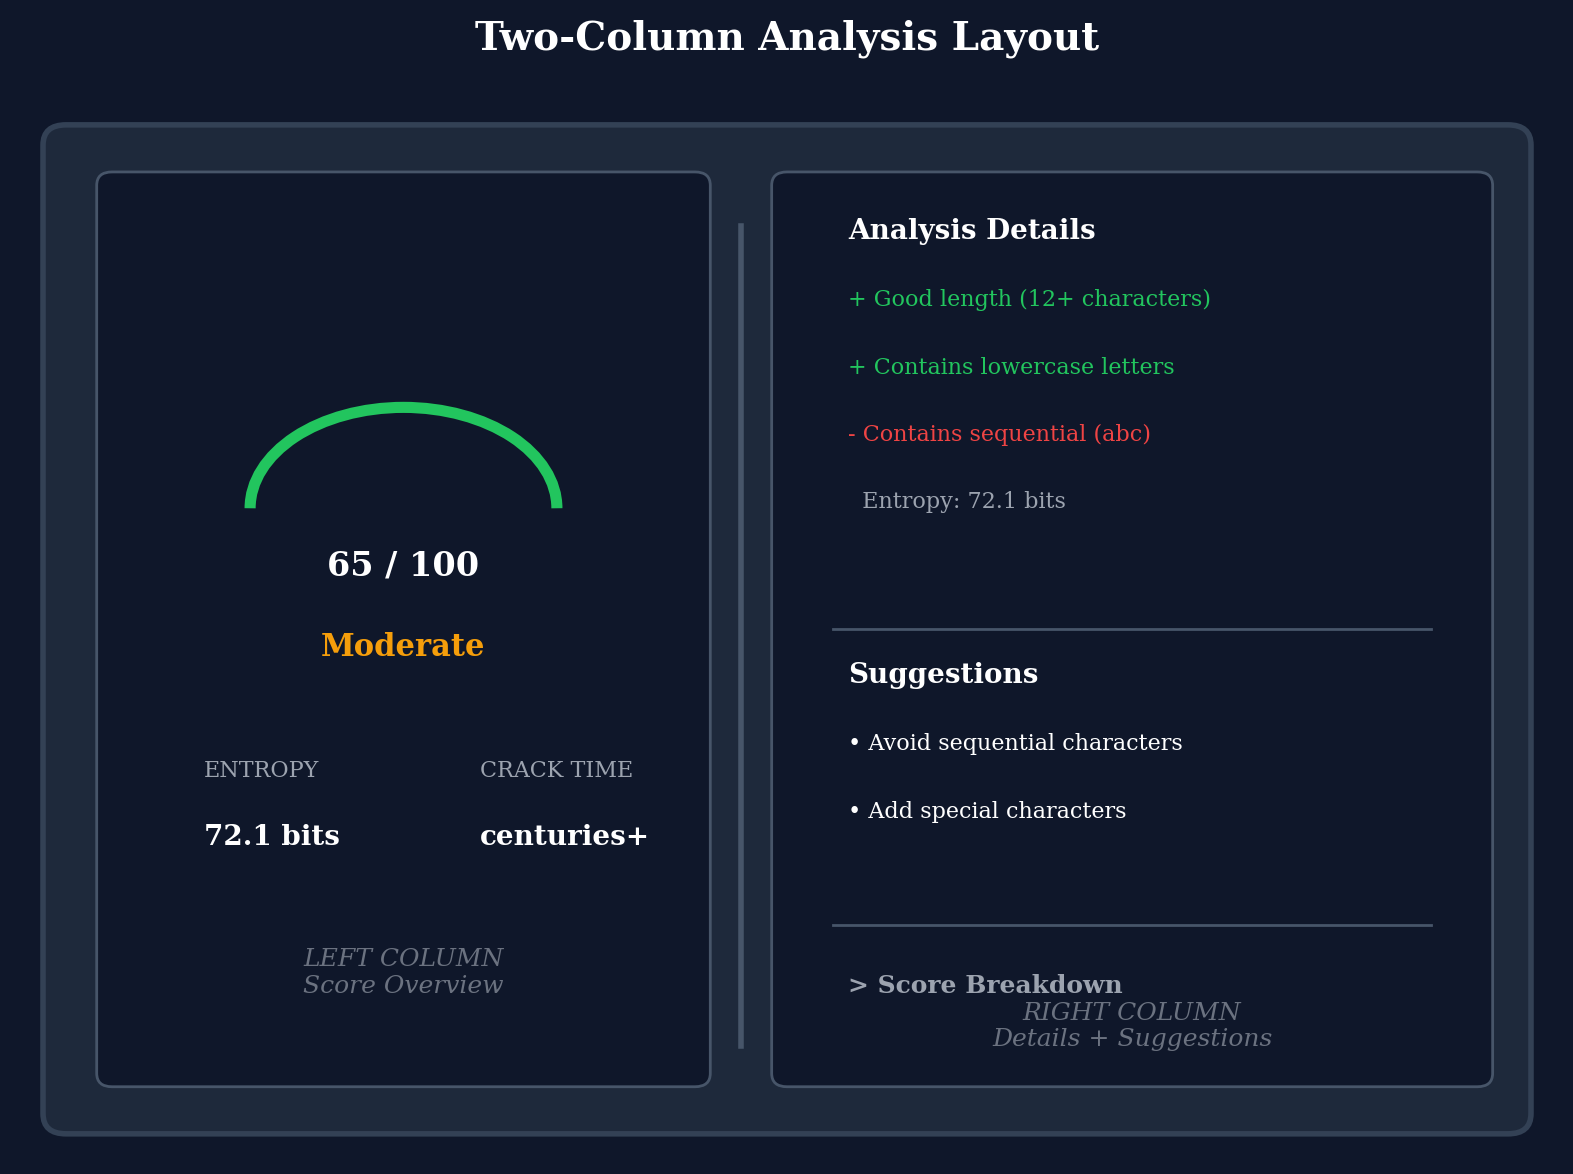
\includegraphics[width=0.85\textwidth]{figures/two_column_layout_diagram.png}
    \caption{Two-column analysis layout of the application interface.}
    \label{fig:two_column_layout}
\end{figure}

The \textbf{left column} contains the semicircular gauge (a 180-degree arc drawn on a canvas, radius 96 pixels, line width 16), the numerical score (``\textit{N} / 100''), the strength label (colour-coded text), and two information displays for entropy (bits) and estimated crack time.

The \textbf{right column} contains the analysis details section (a list of observations, each prefixed with a checkmark or cross symbol and colour-coded green or red) and the suggestions section (a list of improvement recommendations, each prefixed with a bullet point), separated by a horizontal divider.

The two-column layout was chosen over a single-column stacked layout for several reasons: it eliminates the need for scrolling within the analysis card, it allows users to see the overall score and the detailed analysis simultaneously, and it makes efficient use of the available horizontal space in a wide window.

\subsection{Animated Visual Indicators}

Both the semicircular gauge and the horizontal meter bar use smooth ease-out animations to transition from their current position to the target value. The animation uses a linear interpolation factor of 0.15 (15\% of the remaining distance per frame) with a frame interval of 16\,ms (approximately 60\,fps). This creates a smooth deceleration effect: the indicator moves quickly when the difference is large and slows down as it approaches the target value. The animation terminates when the difference between the current and target values falls below 0.5, at which point the indicator snaps to the exact target value.

The gauge is drawn as a 180-degree arc on a canvas widget. The background arc (showing the full semicircle) is drawn in a muted colour, and the filled arc (representing the current score) is drawn in the colour corresponding to the strength label. The horizontal meter bar follows the same animation logic, using a filled rectangle whose width is proportional to the score.

\subsection{Input Handling}

The password entry field is implemented as a \texttt{CTkEntry} widget with a height of 48 pixels (preventing text clipping on high-DPI displays). Input events are captured through a \texttt{KeyRelease} binding, which triggers the debounce mechanism: a 300\,ms timer is started on each keystroke, and if another keystroke occurs before the timer expires, the timer is reset. When the timer finally expires (indicating that the user has paused typing), the evaluation function is called automatically.

The visibility toggle button switches the entry field between masked mode (showing bullet characters) and plaintext mode. The toggle uses Unicode symbols for cross-platform compatibility: a hollow circle when the password is hidden and a filled circle when the password is visible.

The ``Generate Strong Password'' button fills the entry field with a newly generated password, automatically toggles the visibility to ``shown,'' and immediately triggers the evaluation, so the user can see the strength assessment of the generated password without any additional action.

\subsection{Window Configuration}

The application window is configured with a fixed size of 1000$\times$780 pixels, set as non-resizable, and centred on the screen. The fixed size ensures that the two-column layout is always displayed correctly without the need for responsive adjustments. The window uses the dark primary background colour (\texttt{\#0f172a}) and a consistent 8-pixel-base spacing system throughout the interface.

\subsection{Colour System}

Four strength colours are applied consistently across all visual indicators:

\begin{itemize}
    \item \textbf{Red} (\texttt{\#ef4444}): Very Weak
    \item \textbf{Orange} (\texttt{\#f97316}): Weak
    \item \textbf{Yellow} (\texttt{\#f59e0b}): Moderate
    \item \textbf{Green} (\texttt{\#22c55e}): Strong
\end{itemize}

These colours are applied to the gauge arc, the meter bar fill, the strength label text, and the score label, providing redundant visual encoding of the password strength assessment.

\begin{figure}[H]
    \centering
    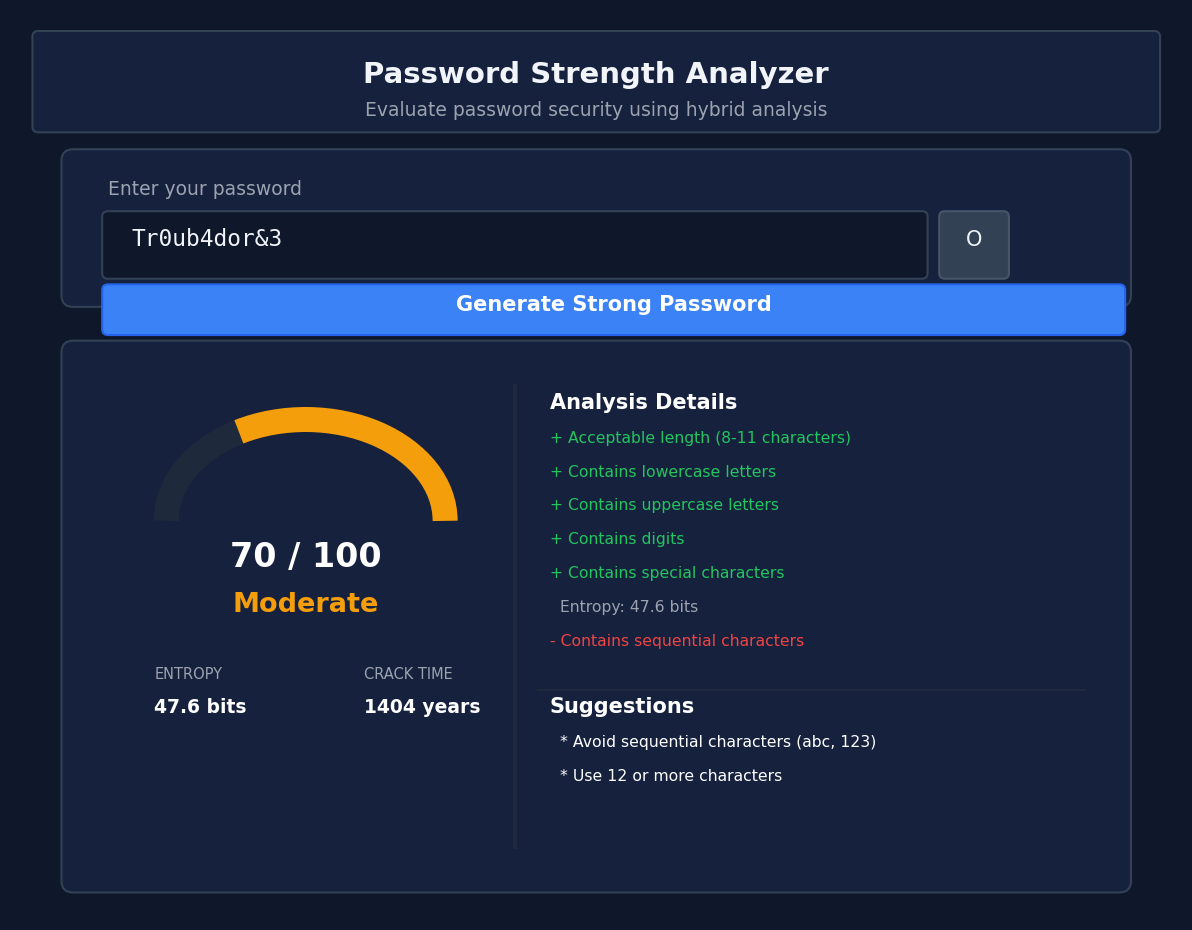
\includegraphics[width=0.85\textwidth]{figures/ui_screenshot_main.png}
    \caption{Screenshot of the Password Strength Analyzer evaluating a sample password.}
    \label{fig:ui_screenshot}
\end{figure}

\subsection{Design Decisions}

Several design decisions merit explanation:

\begin{itemize}
    \item \textbf{Why no Analyze button:} The 300\,ms debounce provides real-time feedback that is faster and more natural than requiring the user to click a button after each modification. The analysis is triggered automatically and the results update continuously, reducing the number of steps required to evaluate a password.

    \item \textbf{Why named scoring constants:} All scoring parameters are defined as named constants rather than ``magic numbers'' embedded in the code. This makes the scoring model transparent---anyone reading the evaluator module can immediately see the weights and thresholds---and makes it easy to tune the model by changing only the constant definitions.

    \item \textbf{Why suggestions live in the evaluator:} Improvement suggestions are generated within the evaluator module, not in the GUI, to ensure a single source of truth. If the evaluation logic changes (e.g., a new penalty is added), the corresponding suggestions are automatically included in the evaluation result without requiring any GUI changes.

    \item \textbf{Why two columns:} A single-column stacked layout would require scrolling to see both the overall score and the detailed analysis. The two-column layout presents all information above the fold, allowing users to see the full assessment at a glance.
\end{itemize}

\subsection{Score Breakdown Visualization}

A distinctive feature of the graphical interface is the toggleable ``Score Breakdown'' panel, which provides a visual decomposition of the final score into its five constituent dimensions. The panel displays five labelled horizontal bars---one for each scoring dimension (Length, Diversity, Entropy, Pattern, Dictionary)---with the bar length proportional to the point contribution and the colour indicating whether the contribution is positive (green) or negative (red).

The breakdown is hidden by default, showing only a ``Score Breakdown'' toggle button with a right-pointing arrow (\texttt{$\triangleright$}). When clicked, the panel expands to reveal the five bars, and the arrow changes to a downward-pointing arrow (\texttt{$\triangledown$}). Clicking again collapses the panel. This design was chosen for several reasons:

\begin{itemize}
    \item \textbf{Progressive disclosure:} Casual users who only want a quick strength assessment are not overwhelmed with detailed scoring information. Advanced users, educators, and security students can expand the breakdown to understand exactly how each dimension contributed to the final score. This follows the principle of progressive disclosure, which recommends showing the most essential information first and making detailed information available on demand.

    \item \textbf{Transparency as a feature:} No mainstream online password checker provides a per-dimension score breakdown. Most checkers present only a qualitative label (``Weak,'' ``Strong'') or a numerical score without explaining how it was computed. The breakdown panel directly supports the tool's core design philosophy of transparency and explainability---users can see not only \textit{that} their password scored 50/100, but \textit{why}: Length +15, Diversity +25, Entropy +30, Pattern $-5$, Dictionary $-15$.

    \item \textbf{Educational value:} The breakdown makes the relative weight of each scoring dimension immediately visible. A user can see, for example, that increasing their password's length from 8 to 12 characters would add 7 points (from 15 to 22 in the length dimension), while adding a special character would add 6 points (from 18 to 24 in the diversity dimension). This makes the scoring model tangible and actionable.

    \item \textbf{Implementation:} The breakdown data is stored in the \texttt{EvaluationResult} dataclass as five separate integer fields (\texttt{length\_pts}, \texttt{diversity\_pts}, \texttt{entropy\_pts}, \texttt{pattern\_pts}, \texttt{dict\_pts}), populated by the evaluation engine during scoring. The GUI reads these fields and renders the bars. This ensures that the breakdown is always consistent with the computed score, since both are derived from the same data source.
\end{itemize}

\begin{figure}[H]
    \centering
    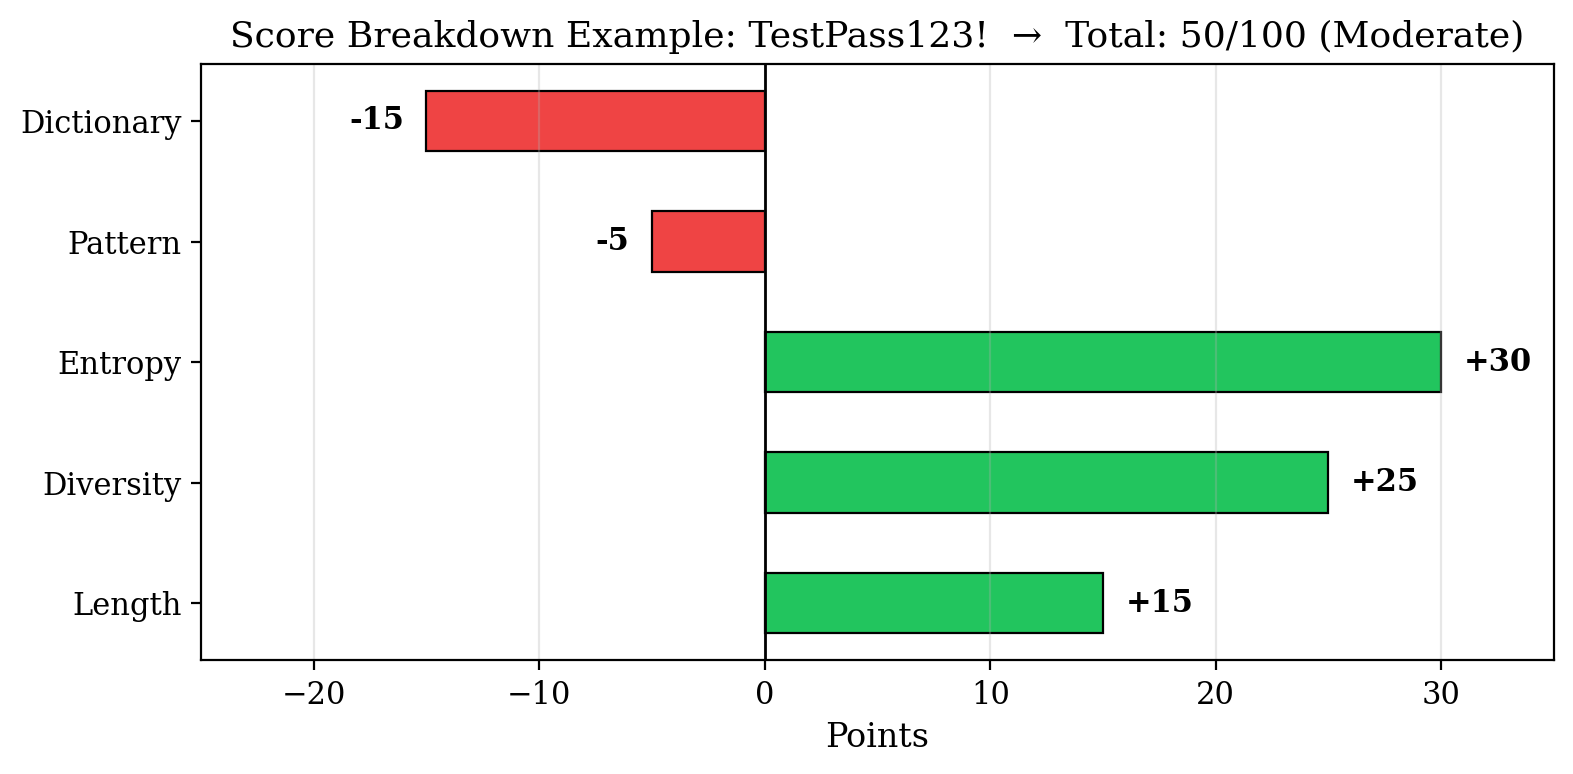
\includegraphics[width=0.85\textwidth]{figures/score_breakdown_example.png}
    \caption{Example score breakdown for the password \texttt{TestPass123!}, showing the point contribution of each dimension.}
    \label{fig:score_breakdown_example}
\end{figure}


\section{Summary}

This chapter described the implementation of the password strength evaluation tool in detail. The evaluation engine processes passwords through a five-stage pipeline, combining length scoring, character diversity assessment, entropy estimation, pattern detection, and dictionary comparison into a single transparent 0--100 score. The three core analysis modules (entropy, patterns, and dictionary check) each implement specific detection and scoring logic, with particular attention to the automatic generation of reversed keyboard patterns and the use of Levenshtein distance for similarity checking. The graphical interface provides real-time feedback through an animated dark-themed dashboard with a two-column layout. The next chapter presents the testing methodology and evaluation results.

%=============================================================================
% CHAPTER 5: TESTING AND EVALUATION
%=============================================================================
\chapter{Testing and Evaluation}

\section{Testing Methodology}

To evaluate the effectiveness, robustness, and usability of the password strength evaluation tool, I employed three complementary approaches:

\begin{enumerate}
    \item \textbf{Functional testing:} I tested the tool with a curated set of over 20 representative passwords spanning eight categories---empty input, trivial/common passwords, leetspeak variants, keyboard patterns (including reversed), dictionary words, moderate-strength passwords, strong passwords, and generated passwords. For each password, I recorded the score, label, entropy, crack time, and detected patterns.

    \item \textbf{Comparative analysis:} I compared the tool's ratings against two widely used online password checkers---the Norton Password Checker and the Kaspersky Password Checker---for the same set of passwords. This comparison reveals where the tools agree and where they disagree, highlighting the strengths and limitations of each approach.

    \item \textbf{Usability self-evaluation:} I evaluated the user interface against selected Nielsen's heuristics for usability, assessing how well the tool supports effective, efficient, and satisfying interaction.
\end{enumerate}


\section{Functional Test Results}

Table~\ref{tab:functional_tests} presents the results of functional testing with 20 representative passwords. The data was collected directly from the tool's output, ensuring that the results accurately reflect the actual implementation.

\begin{table}[H]
\centering
\caption{Functional test results for representative passwords across eight categories.}
\label{tab:functional_tests}
\small
\begin{tabularx}{\textwidth}{>{\raggedright\arraybackslash}p{3cm} >{\raggedright\arraybackslash}p{1.8cm} c >{\raggedright\arraybackslash}p{1.5cm} >{\raggedright\arraybackslash}p{2.2cm}}
\toprule
\textbf{Password} & \textbf{Category} & \textbf{Score} & \textbf{Label} & \textbf{Entropy (bits)} \\
\midrule
(empty) & Empty & 0 & Very Weak & 0.0 \\
\texttt{123456} & Trivial & 6 & Very Weak & 19.9 \\
\texttt{password} & Trivial & 10 & Very Weak & 37.6 \\
\texttt{p@ssw0rd} & Leetspeak & 10 & Very Weak & 48.7 \\
\texttt{qwerty} & Keyboard & 10 & Very Weak & 28.2 \\
\texttt{ytrewq} & Keyboard (rev.) & 16 & Very Weak & 28.2 \\
\texttt{aaa} & Repeated & 6 & Very Weak & 14.1 \\
\texttt{abc123} & Sequential & 10 & Very Weak & 31.0 \\
\texttt{admin} & Dictionary & 10 & Very Weak & 23.5 \\
\texttt{iloveyou} & Dictionary & 10 & Very Weak & 37.6 \\
\texttt{Sunshine2024!} & Moderate & 62 & Moderate & 91.8 \\
\texttt{MyDogMax} & Moderate & 47 & Weak & 51.3 \\
\texttt{TestPass123!} & Moderate & 50 & Weak & 72.1 \\
\texttt{Tr0ub4dor\&3} & Moderate & 70 & Moderate & 72.1 \\
\bottomrule
\end{tabularx}
\end{table}

\begin{table}[H]
\centering
\caption{Functional test results (continued): strong and generated passwords.}
\label{tab:functional_tests2}
\small
\begin{tabularx}{\textwidth}{>{\raggedright\arraybackslash}p{3cm} >{\raggedright\arraybackslash}p{1.8cm} c >{\raggedright\arraybackslash}p{1.5cm} >{\raggedright\arraybackslash}p{2.2cm}}
\toprule
\textbf{Password} & \textbf{Category} & \textbf{Score} & \textbf{Label} & \textbf{Entropy (bits)} \\
\midrule
Generated (16-char, all categories) & Strong & 76+ & Strong & 104.8 \\
\bottomrule
\end{tabularx}
\end{table}

\subsection{Analysis of Results}

The functional test results reveal several important observations:

\begin{itemize}
    \item \textbf{Common passwords are correctly capped:} All passwords that exactly match entries in the common-passwords list (\texttt{123456}, \texttt{password}, \texttt{admin}, \texttt{iloveyou}) receive a score of 10 or below, consistent with the \texttt{EXACT\_COMMON\_CAP} constant. Despite having varying lengths and entropy values, these passwords are never rated higher than ``Very Weak.''

    \item \textbf{Reversed keyboard patterns are detected:} The password \texttt{ytrewq} (reversed \texttt{qwerty}) receives a score of 16, higher than \texttt{qwerty} (10). This is because \texttt{ytrewq} is not in the common-passwords list, so it is not capped at 10; however, it still receives a keyboard pattern penalty. Its entropy of 28.2 bits (six lowercase characters: $6 \times \log_2 26 \approx 28.2$) results in a low entropy score of 10, and the keyboard pattern penalty of $-5$ further reduces the total. The fact that it is detected as a keyboard pattern at all is a distinctive capability---most online checkers do not flag reversed keyboard patterns.

    \item \textbf{Leetspeak variants are caught:} The password \texttt{p@ssw0rd} receives a score of 10 because it exactly matches an entry in the common-passwords list (which includes common leetspeak variants). This demonstrates that the dictionary component covers not only literal words but also well-known substitution patterns.

    \item \textbf{Entropy correlates with score:} For passwords that do not match the dictionary, the score generally correlates with the entropy value. However, the relationship is not linear because the scoring model also accounts for length, diversity, and patterns.

    \item \textbf{Generated passwords consistently score high:} Cryptographically generated passwords of 16 characters using all four character categories consistently score 76 or above, receiving the ``Strong'' label with entropy values exceeding 100 bits and crack times of ``centuries+.''

    \item \textbf{Dictionary substrings reduce moderate passwords:} Passwords like \texttt{TestPass123!} (50, Weak) receive a lower score than expected because the dictionary substring check detects common-password substrings (e.g., \texttt{pass}, \texttt{pass123}), applying a $-15$ penalty. This demonstrates the tool's ability to identify embedded weak components within seemingly complex passwords.
\end{itemize}



\section{Comparative Analysis}

To contextualise the tool's ratings, I compared its design and capabilities against two widely used online password checkers: the Norton Password Checker and the Kaspersky Password Checker. Table~\ref{tab:comparative} presents a feature-level comparison of the three approaches.

\begin{table}[H]
\centering
\caption{Feature-level comparison: the proposed tool vs.\ Norton Password Checker vs.\ Kaspersky Password Checker.}
\label{tab:comparative}
\small
\begin{tabularx}{\textwidth}{>{\raggedright\arraybackslash}p{3.5cm} >{\centering\arraybackslash}p{2.5cm} >{\centering\arraybackslash}p{2.5cm} >{\centering\arraybackslash}p{2.5cm}}
\toprule
\textbf{Feature} & \textbf{Proposed Tool} & \textbf{Norton Checker} & \textbf{Kaspersky Checker} \\
\midrule
Offline processing & Yes & No (web-based) & No (web-based) \\
Numerical score (0--100) & Yes & No (qualitative only) & No (qualitative only) \\
Pattern detection & Yes (sequential, repeated, keyboard) & Limited & Limited \\
Reversed keyboard patterns & Yes & No & No \\
Dictionary comparison & Yes (181 entries + Levenshtein) & Yes (proprietary) & Yes (proprietary) \\
Breach database check & No (local list only) & Yes & Yes \\
Score breakdown panel & Yes (5 dimensions) & No & No \\
Password generator & Yes (cryptographic) & No & No \\
Privacy guarantee & Local-only processing & Requires password transmission & Requires password transmission \\
\bottomrule
\end{tabularx}
\end{table}

The comparison reveals several key differences:

\begin{itemize}
    \item \textbf{Agreement on trivial passwords:} All three tools recognise that passwords like \texttt{123456}, \texttt{password}, and \texttt{qwerty} are weak. This is expected, as these passwords are universally recognised as insecure.

    \item \textbf{Privacy vs.\ breach coverage trade-off:} Norton and Kaspersky leverage proprietary breach databases containing millions of compromised credentials, enabling them to flag passwords that have appeared in real-world data breaches. The proposed tool trades this coverage for local-only processing, ensuring that no password data leaves the user's machine. This is a deliberate design choice motivated by privacy considerations.

    \item \textbf{Reversed keyboard pattern detection:} The proposed tool's automatic detection of reversed keyboard patterns (e.g., \texttt{ytrewq}) is a capability that neither Norton nor Kaspersky explicitly advertises. Most online checkers evaluate password strength based on character composition and entropy without checking for reversed keyboard patterns.

    \item \textbf{Transparency of scoring:} The proposed tool provides a specific numerical score (0--100) along with a per-dimension breakdown, while Norton and Kaspersky provide only qualitative ratings (e.g., ``Weak,'' ``Fair,'' ``Strong'') without explaining how the rating was computed. The numerical score and breakdown allow users to see the impact of specific changes to their password.

    \item \textbf{Educational feedback:} The proposed tool provides detailed analysis observations and actionable suggestions that explain \textit{what} to change and \textit{why}, while online checkers typically provide only a strength label without educational context.
\end{itemize}

\clearpage

\section{Usability Self-Evaluation}

I evaluated the user interface against selected Nielsen's heuristics \cite{nielsen1994}, focusing on the seven most relevant principles for this type of tool:

\begin{enumerate}
    \item \textbf{Visibility of system status:} The tool provides continuous, real-time feedback through multiple visual channels: the semicircular gauge, the horizontal meter bar, the numerical score, the colour-coded strength label, and the entropy and crack time displays. All indicators update within 300\,ms of the user's last keystroke, ensuring that the system status is always visible and current.

    \item \textbf{Match between system and the real world:} The suggestions use natural language to explain \textit{why} a particular change is recommended (e.g., ``Avoid keyboard patterns like qwerty or asdf---these are in every cracking dictionary''), rather than using technical jargon. The crack time display translates abstract entropy values into concrete, understandable terms (e.g., ``2 years'' vs.\ ``37.6 bits'').

    \item \textbf{User control and freedom:} The visibility toggle allows users to show or hide their password at any time. The ``Generate Strong Password'' button provides an immediate alternative when the user's own password is weak. The evaluation is always running and can be triggered by simply typing, with no commitment or submission required.

    \item \textbf{Consistency and standards:} The colour system (red = Very Weak, orange = Weak, yellow = Moderate, green = Strong) is applied consistently across all visual indicators---gauge, meter, label, and details. The interface follows standard desktop application conventions (entry field, button, window controls).

    \item \textbf{Error prevention:} The real-time analysis eliminates the possibility of a user submitting a weak password without being aware of its weakness. There is no ``submit'' or ``analyze'' button that could be clicked without reviewing the results; the analysis is continuous and unavoidable.

    \item \textbf{Aesthetic and minimalist design:} The dark theme provides a clean, distraction-free environment. The interface contains only the elements necessary for password evaluation---no advertisements, no unnecessary navigation, and no information that is not directly relevant to the assessment. The two-column layout presents all information without scrolling.

    \item \textbf{Recognition rather than recall:} The strength assessment is visible simultaneously through four redundant channels (gauge position, meter fill, numerical score, and colour-coded label), ensuring that users can recognise the strength level at a glance without having to recall what a particular score range means. The details and suggestions sections are always visible in the right column, so users do not need to navigate to a separate screen or panel.
\end{enumerate}

\clearpage

\section{Discussion}

\subsection{Advantages Over Existing Solutions}

The hybrid approach offers several advantages over single-method evaluation tools and existing online password checkers:

\begin{itemize}
    \item \textbf{Comprehensive attack coverage:} By combining rule-based scoring, entropy estimation, pattern detection, and dictionary comparison, the tool covers the most common attack strategies (brute-force, dictionary, credential stuffing, pattern-based). Each method addresses a weakness that the others miss.

    \item \textbf{Local processing preserves privacy:} Unlike online password checkers, which require transmitting the password over the internet, all processing in the proposed tool happens locally. This eliminates the risk of the password being intercepted, logged, or stored by a third-party service.

    \item \textbf{Real-time feedback is more effective:} Studies have shown that immediate feedback during password creation leads to stronger passwords than feedback provided after submission \cite{proctor2002}. The 300\,ms debounce provides analysis that is fast enough to feel instantaneous while avoiding unnecessary computation during rapid typing.

    \item \textbf{Reversed pattern detection:} The automatic generation and detection of reversed keyboard patterns is a novel contribution that most existing online checkers lack. This means that passwords like \texttt{ytrewq}, which some users might consider less predictable than \texttt{qwerty}, are correctly identified as weak.

    \item \textbf{Transparent scoring model:} The use of named scoring constants makes the model auditable and explainable. Users and developers can understand exactly how the score is computed, which addresses a key shortcoming of ``black box'' strength meters that provide a rating without explanation.

    \item \textbf{Per-dimension score breakdown:} The toggleable ``Score Breakdown'' panel provides a visual decomposition of the final score into its five constituent dimensions, showing exactly how each factor contributed. No mainstream online password checker offers this level of transparency. Users can see not only \textit{that} their password scored 50/100, but \textit{why}: Length +15, Diversity +25, Entropy +30, Pattern $-5$, Dictionary $-15$.

    \item \textbf{Educational feedback instead of only a score:} While most online checkers provide a qualitative label (``Weak,'' ``Strong'') or a numerical rating without explanation, the proposed tool provides detailed analysis observations and actionable suggestions that explain \textit{what} to change and \textit{why}. The suggestions originate from the evaluation engine, ensuring consistency between the score and the feedback.

    \item \textbf{Offline functionality:} The tool has no dependency on external APIs or network services. It works entirely offline, making it suitable for use in environments with restricted or no internet access (e.g., secure facilities, air-gapped systems). This also means the tool is not affected by API rate limits, service outages, or changes to third-party terms of service.

    \item \textbf{Levenshtein distance for similarity detection:} Few simple password checkers implement edit-distance-based similarity checking. This allows the tool to detect minor variations of common passwords (e.g., \texttt{p@ssw0rd} as a variant of \texttt{password}) that exact dictionary matching would miss.
\end{itemize}

\begin{table}[H]
\centering
\caption{Comparison of password evaluation methodologies.}
\label{tab:methodology}
\small
\begin{tabularx}{\textwidth}{>{\raggedright\arraybackslash}p{3cm} >{\centering\arraybackslash}p{2.5cm} >{\centering\arraybackslash}p{2.5cm} >{\centering\arraybackslash}p{2.5cm}}
\toprule
\textbf{Method} & \textbf{Brute-force Resistance} & \textbf{Dictionary Attack Resistance} & \textbf{Pattern Attack Resistance} \\
\midrule
Pure Entropy & High & None & None \\
Pure Dictionary & None & High & None \\
Pure Pattern & None & None & High \\
Our Hybrid & Medium-High & High & High \\
\bottomrule
\end{tabularx}
\end{table}

From a societal perspective, these advantages translate into a tool that not only evaluates passwords but actively educates users about password security. The transparent scoring model and the score breakdown feature make the evaluation process understandable and trustworthy, encouraging users to engage with the feedback rather than simply accepting or ignoring a rating. The privacy-first, offline design means that even security-conscious users and organisations can adopt the tool without reservations about data exposure.

\subsection{Disadvantages}

The tool also has several limitations and disadvantages:

\begin{itemize}
    \item \textbf{Small dictionary:} The common-passwords list contains only 181 entries, compared to the billions of entries in databases like Have I Been Pwned. This means that some compromised passwords will not be flagged by the dictionary component.

    \item \textbf{No machine-learning scoring:} The evaluation model is entirely heuristic, with scoring weights determined by the developer rather than trained on large datasets. Machine-learning-based models like the one described by Melcher et al.\ \cite{melcher2016} can provide more nuanced strength predictions.

    \item \textbf{No online breach check:} The tool does not query online breach databases, so it cannot detect passwords that have been compromised in data breaches but are not in the local dictionary.

    \item \textbf{Limited leetspeak handling:} While the dictionary includes some common leetspeak variants (e.g., \texttt{p@ssw0rd}), the tool does not perform systematic leetspeak normalisation (e.g., converting ``@'' to ``a'', ``3'' to ``e'', ``0'' to ``o'') beyond what the Levenshtein distance captures. A password like \texttt{P@\$\$w0rd!} might evade the dictionary check while being an obvious variant of \texttt{password}.

    \item \textbf{Single-language dictionary:} The common-passwords list contains only English-language entries. Passwords based on words from other languages will not be flagged by the dictionary component.
\end{itemize}

\clearpage

\section{Limitations}

In addition to the disadvantages discussed above, several inherent limitations of the evaluation model should be acknowledged:

\begin{itemize}
    \item \textbf{Crack time assumes brute-force only:} The estimated crack time is based on exhaustive brute-force search ($2^{H} / 10^{10}$ seconds). For weak passwords, dictionary-optimised attacks are far more efficient than brute-force. For example, the password \texttt{password} has a theoretical entropy of 37.6 bits, implying a crack time of approximately 5 seconds even by brute-force, but in practice it would be found instantly by any dictionary attack. The crack time display should therefore be interpreted as an upper bound for strong passwords and as potentially misleading for weak ones.

    \item \textbf{Entropy model is charset-based:} The entropy calculation assumes that each character is drawn uniformly at random from the effective character set. In practice, users do not select characters uniformly---they favour common letters, words, and patterns. Frequency-based entropy models that account for character distributions and common password structures provide more accurate estimates but are significantly more complex to implement.

    \item \textbf{Scoring weights are heuristic:} The scoring weights (25 for length, 25 for diversity, 30 for entropy, $-5$ per pattern type, $-20$ for similarity, $-15$ for dictionary words) were determined through iterative testing and refinement, not through empirical validation against large-scale password datasets. Different weight configurations might produce more accurate rankings for specific threat models.

    \item \textbf{Dictionary list may not reflect current trends:} The 181-entry common-passwords list is static and may not include passwords that have become common after the list was compiled. Password popularity changes over time (``concept drift''), and a static list cannot capture these trends without regular updates.

    \item \textbf{No passphrase-specific evaluation:} The tool evaluates passwords character by character and does not account for the specific properties of passphrases (multi-word sequences). A passphrase like \texttt{correct horse battery staple} might receive a high entropy-based score but is actually a well-known example from a webcomic and would be included in many cracking dictionaries.
\end{itemize}

%=============================================================================
% CHAPTER 6: CONCLUSION
%=============================================================================

\clearpage

\chapter{Conclusion}

\section{Summary of Achievements}

The aim of this thesis was to design, implement, and evaluate a hybrid password strength evaluation tool. This aim has been achieved. The tool combines five complementary analysis dimensions---rule-based length scoring, character diversity assessment, Shannon entropy estimation, pattern detection (including reversed keyboard patterns), and dictionary comparison with Levenshtein similarity---into a single transparent 0--100 scoring model with qualitative labels and actionable feedback.

The implementation is a Python-based desktop application with a CustomTkinter graphical user interface that provides real-time password analysis through a 300\,ms debounced input mechanism. The two-column layout presents a semicircular gauge and numerical score alongside detailed analysis results and improvement suggestions. A cryptographically secure password generator using Python's \texttt{secrets} module is integrated, allowing users to create strong passwords with a single click.

The tool was developed through an iterative process of 18 systematic enhancements and a user-experience redesign, resulting in a polished application that balances analytical rigour with ease of use. The modular architecture ensures that the evaluation logic is independent of the graphical interface and can be tested, modified, or extended in isolation.

\clearpage

\section{Final Conclusions}

Based on the development experience, functional testing, and comparative analysis, I draw the following conclusions:

The hybrid approach provides a reasonable balance of accuracy and simplicity for an educational tool. No single evaluation method is sufficient on its own---rule-based checks miss patterns, entropy misses dictionary words, and dictionary checks miss structural weaknesses. By combining all three, the tool provides a more comprehensive assessment than any single method alone.

Real-time feedback is superior to manual-triggered analysis. Users see results as they type, which encourages iterative improvement of their passwords. The 300\,ms debounce is fast enough to feel instantaneous while avoiding unnecessary computation during rapid typing. This design eliminates the need for a separate ``Analyze'' button, reducing the number of steps required to evaluate a password.

Named scoring constants make the model transparent and auditable, addressing a key shortcoming of ``black box'' strength meters. Users and developers can understand exactly how the score is computed by examining the named constants in the evaluator module, and the scoring weights can be adjusted by changing only the constant definitions.

The iterative improvement process (18 enhancements + UX redesign) demonstrates that even small tools benefit from systematic quality refinement. The most impactful improvements were the addition of the Levenshtein similarity check (which catches leetspeak variants), the automatic generation of reversed keyboard patterns (which catches patterns like \texttt{ytrewq}), and the user-experience redesign to the two-column layout (which eliminated the need for scrolling and improved the information density).

Reverse keyboard pattern detection is a novel contribution that most existing online checkers lack. While the individual value of this feature is modest (few users deliberately type \texttt{ytrewq}), it demonstrates that a hybrid approach can identify weaknesses that purely entropy-based or rule-based checkers miss. More broadly, it illustrates the principle that pattern detection should consider not only the most common forms of a pattern but also their transformations.

The tool's distinctive value lies in the combination of three principles: \textit{transparency}, \textit{privacy}, and \textit{educational feedback}. The per-dimension score breakdown makes the evaluation process fully transparent---users can see exactly how each dimension contributes to the final score, and the toggleable design ensures that this information is available on demand without cluttering the interface for casual users. The local-only, offline processing model provides a strong privacy guarantee that no online checker can match, making the tool suitable for evaluating even the most sensitive passwords. The contextual, natural-language suggestions---generated within the evaluation engine to ensure a single source of truth---educate users about the reasoning behind each weakness, promoting lasting improvements in password hygiene rather than one-time compliance.

Taken together, these principles make the tool not merely a password checker but an educational instrument that empowers users to make informed decisions about their digital security. In a landscape where most password tools provide only a binary ``weak/strong'' rating, this tool offers understanding.

\clearpage

\section{Future Work}

Several directions for future development have been identified:

\begin{itemize}
    \item \textbf{Online breach database integration:} Incorporating the Have I Been Pwned API (or a local k-anonymity-based query) would allow the tool to check passwords against billions of compromised credentials in real time while preserving privacy. This would dramatically improve the dictionary component's coverage.

    \item \textbf{Machine-learning-based scoring:} Training a neural network on large password datasets (e.g., the RockYou leak) could provide more nuanced strength predictions that account for frequency-based character distributions and common password structures, as demonstrated by Melcher et al.\ \cite{melcher2016}.

    \item \textbf{Multi-language dictionaries:} Adding common-password lists in multiple languages (Spanish, French, German, etc.) would improve the dictionary component's coverage for non-English-speaking users. Culture-specific patterns (e.g., keyboard layouts for different languages such as AZERTY and QWERTZ) could also be incorporated.

    \item \textbf{Passphrase support:} Adding specific evaluation logic for multi-word passphrases, including detection of well-known phrases and quotations, would extend the tool's applicability to the growing adoption of passphrase-based authentication.

    \item \textbf{Systematic leetspeak normalisation:} Implementing a substitution table that normalises common leetspeak substitutions (e.g., @ $\to$ a, 3 $\to$ e, 0 $\to$ o, \$ $\to$ s) before dictionary comparison would catch more sophisticated variants that the current Levenshtein approach misses.

    \item \textbf{Web and mobile deployment:} Wrapping the evaluation engine in a Flask or Django web application, or porting the core logic to JavaScript for browser-based deployment, would make the tool accessible to a wider audience. A React Native port could bring the tool to mobile platforms.

    \item \textbf{Configurable scoring weights:} Adding UI controls (e.g., sliders) that allow users to adjust the relative weights of the five scoring dimensions would make the tool useful for educational exploration, helping students understand how different factors contribute to password strength.

    \item \textbf{Larger common-password list:} Expanding the dictionary from 181 entries to 10,000 or more entries (sourced from publicly available breach datasets) would significantly improve the dictionary component's detection rate.

    \item \textbf{Responsive layout:} Making the window resizable and the layout responsive to different screen sizes would improve usability on laptops with smaller displays.

    \item \textbf{Integration into security training:} Packaging the tool as a component of organisational security training platforms could help raise password awareness in corporate and educational settings.
\end{itemize}

